\documentclass{article}
\usepackage{float}
\usepackage[eandd,nonatbib]{neurips_2026}
\usepackage[utf8]{inputenc}
\usepackage[T1]{fontenc}
\usepackage[numbers,sort&compress]{natbib}
\usepackage{hyperref}
\hypersetup{hidelinks}
\usepackage{url}
\usepackage{booktabs}
\usepackage{amsfonts}
\usepackage{amsmath}
\usepackage{amssymb}
\usepackage{nicefrac}
\usepackage{microtype}
\usepackage{xcolor}
\usepackage{graphicx}
\usepackage{tabularx}
\usepackage{multirow}
\usepackage{array}
\usepackage{placeins}
\usepackage{wrapfig}
\usepackage{tikz}
\usepackage{capt-of}
\usepackage{listings}
\usepackage{comment}
\usepackage{enumitem}
\usetikzlibrary{arrows.meta,positioning,fit}
\lstset{
  basicstyle=\ttfamily\footnotesize,
  breaklines=true,
  columns=fullflexible,
  keepspaces=true
}

% Loosen float placement slightly to avoid half-empty pages.
\setlength{\textfloatsep}{10pt plus 2pt minus 2pt}
\setlength{\floatsep}{8pt plus 2pt minus 2pt}
\setlength{\intextsep}{8pt plus 2pt minus 2pt}
\setlength{\abovecaptionskip}{6pt}
\setlength{\belowcaptionskip}{2pt}
\renewcommand{\topfraction}{0.9}
\renewcommand{\bottomfraction}{0.8}
\renewcommand{\textfraction}{0.07}
\renewcommand{\floatpagefraction}{0.8}

% Framework name command — update here only if the style file does not define it.
\providecommand{\frameworkname}{Our framework}
\providecommand{\model}[1]{\emph{#1}}
\providecommand{\metric}[1]{\textsc{#1}}
\newcommand{\deltaplan}[1]{\begingroup\setlength{\fboxsep}{1.2pt}\colorbox{yellow!25}{\strut #1}\endgroup}

\title{Beyond Sequential Plans: A Three-Facet Evaluation of Agentic Planning under Plan-Preserving Perturbation}

\author{Anonymous Authors \\
Anonymous Institution \\
\emph{anonymous@anonymous.edu}}

\begin{document}

\maketitle
\begin{abstract}
A correct final answer can hide a broken plan, and a wrong final answer can hide a correct one.
Evaluating LLM agents only by their final answers therefore tells us little about \emph{where} they fail.
We propose evaluating three facets of agentic behavior separately---plan structural fidelity, tool invocation accuracy, and end-task answer correctness---and build a benchmark on top of GAIA that supports all three on the same task.
We add an explicit tool layer and a dependency-aware planning reference whose reordered alternatives are validated by a behavior-preserving replay filter.
Across seven open-weight models spanning $50\times$ in parameter count, every single model recovers more dependencies under our augmented reference, with EdgeF1 lifting by $+45.4\%$ relative on the subset where reordering matters most---roughly three times the lift we see when this signal is averaged across all tasks.
Because the three facets rank models differently---the largest open-weight model (675B) scores worse on final answers than a 31B model in the same pool---the three facets together reveal capability gaps that a single answer-rate would otherwise conflate.
Code and data are available at \url{https://github.com/anonymousllmplanning/llm-planning}.
\end{abstract}

\section{Introduction}
Large language models are increasingly deployed as agents that decompose requests, call external tools, and synthesize final answers from intermediate observations~\cite{10.1145/3586183.3606763,hong2024metagpt,shen2023hugginggpt}. 
Chain-of-Thought~\cite{CoT, gao-etal-2025-efficient}, Tree-of-Thought~\cite{yao2024tree, ni-etal-2025-tree}, and ReAct~\cite{yao2022react,shen2026thinking} all share a common premise: before an agent executes a task, it must first form a plan that organizes subgoals, dependencies, and tool-facing actions.
The plan is therefore an evaluable object, distinct from the final answer it produces.

But a benchmark that scores only the final answer cannot tell whether a failure came from a broken plan, a malformed tool call, or downstream answer synthesis---and a correct answer can mask a brittle plan that happened to succeed. 
We argue that a useful benchmark for agentic systems should evaluate at least three facets separately: (A) \emph{Plan Structural Fidelity},  the dependency structure the model attributes to the task before execution; (B) \emph{Tool Invocation Accuracy}, whether selected tools and grounded arguments cover the evidence-gathering actions the task requires; and (C) \emph{End-Task Answer Correctness}, whether the submitted answer is accepted under standard evaluation.

Existing structural metrics already provide useful primitives:  \metric{NodeF1} and \metric{EdgeF1}~\cite{shen2024taskbench,gabriel2024advancing} measure whether a predicted planning graph recovers the labeled nodes and dependencies of a gold reference.
But the gold reference itself is the bottleneck: when it is a single serialized chain, incidental ordering looks like a required dependency, and plans that respect the underlying dependency structure but reorder independent branches are penalized. 
We address this by augmenting GAIA~\cite{mialon2023gaia}, which provides realistic multimodal tasks with verifiable final answers but primarily chain-style supervision. We add an explicit tool layer and convert each chain into a dependency DAG (directed acyclic graph) whose reordered alternatives are validated by a behavior-preserving replay filter, so that plans matching any dependency-preserving reordering can receive credit.
The synthesized dependencies are validated by a three-annotator spot-check (98.4\% edge correctness).


Across seven open-weight models spanning $50\times$ in parameter count, every single model recovers more dependencies under our augmented reference, with EdgeF1 lifting by $+45.4\%$ relative on the subset where reordering matters most---roughly three times the lift seen when the signal is averaged across the full benchmark. 
The three facets rank models differently: the largest open-weight model in our pool (675B) scores worse on final answers than a 31B model from the same pool, and once tool execution is controlled, planning quality predicts answer correctness only weakly and model-dependently. The takeaway is that planning, tool use, and answer correctness are related but not interchangeable capabilities, and a benchmark that scores them separately reveals capability differences that a single answer-rate would otherwise conflate.


This paper makes three contributions:
\begin{itemize}[noitemsep, topsep=2pt, leftmargin=*]
    \item \textbf{A three-facet evaluation framework} that jointly scores plan structural fidelity, tool invocation accuracy, and end-task answer correctness on the same task instance, keeping downstream synthesis separable from planning and tool-use errors.
    \item \textbf{A GAIA-derived benchmark} that adds an explicit tool layer and dependency-aware planning reference to Native GAIA, with reordered alternatives validated by a behavior-preserving replay filter, turning an answer-centric benchmark into a unified planning-execution-answer resource.
    \item \textbf{A systematic open-weight evaluation} showing that model rankings differ across the three facets, that augmentation lifts dependency recovery for every model evaluated (most strongly on multi-order-rich tasks), and that planning--answer correlation conditional on clean tool execution is mildly positive but heterogeneous.
\end{itemize}


\section{Related Work}
\label{sec:related-work}

\paragraph{Reasoning to tool-augmented planning.} Recent work has transformed LLMs into tool-augmented agents that solve requests through explicit intermediate reasoning and external actions~\cite{CoT,yao2022react,yao2024tree}. Once reasoning is externalized into a multi-step plan that drives tool invocation, the plan itself becomes an evaluable object rather than a hidden by-product behind final task success.

\paragraph{Benchmarks for tool use and task automation.} Benchmarks for tool use have evolved from API-centric function-calling tests~\cite{patil2023gorilla,qin2023toolllm} toward structured evaluations of task automation. TaskBench introduces Tool Graphs to model dependency structure between tools~\cite{shen2024taskbench}; GTA emphasizes human-written queries with real deployed tools and multimodal inputs~\cite{wang2024gta}; UltraTool expands evaluation to the broader lifecycle of planning, creation, and usage~\cite{huang2024ultratool}. Answer-centric benchmarks such as GAIA measure end-to-end completion under realistic multimodal settings but do not isolate whether success or failure originated in planning, execution, or final synthesis~\cite{mialon2023gaia}.

\paragraph{Planning-aware evaluation and our setting.} A more recent line of work evaluates planning and execution as distinct components of agentic behavior~\cite{gabriel2024advancing,ahn2026orchestrationbench}. Our setting differs in two ways. First, we score the model's planning graph separately from the realized tool trace while retaining GAIA's verifiable answer target, so the same record supports all three facets. Second, plan structural evaluation uses a dependency-preserving augmented reference set rather than a single canonical chain, so that plans reordering independent branches are credited rather than penalized. 
Table~\ref{tab:related-work-comparison} summarizes the dimensions that most directly motivate this setup.

\begin{table}[b]
\centering
\setlength{\tabcolsep}{0.55pt}
\scriptsize
%\resizebox{\linewidth}{!}{%
\makebox[\linewidth][c]{%
\begin{tabular}{lccccccc}
\toprule
Benchmark & Plan Graph & Tool-Use Eval. & Executed Trace & Realistic Tasks & Component Eval. & Dependency/Order Refs. & Flexible-Order Scoring \\
\midrule
TaskBench \cite{shen2024taskbench} & $\checkmark$ & $\checkmark$ & $\times$ & $\times$ & $\checkmark$ & $\checkmark$ & $\times$ \\
Advancing Agentic Systems \cite{gabriel2024advancing} & $\checkmark$ & $\checkmark$ & $\checkmark$ & $\times$ & $\checkmark$ & $\checkmark$ & $\times$ \\
GAIA \cite{mialon2023gaia} & $\times$ & $\times$ & $\times$ & $\checkmark$ & $\times$ & $\times$ & $\times$ \\
GTA \cite{wang2024gta} & $\times$ & $\checkmark$ & $\checkmark$ & $\checkmark$ & $\times$ & $\times$ & $\times$ \\
UltraTool \cite{huang2024ultratool} & $\checkmark$ & $\checkmark$ & $\times$ & $\checkmark$ & $\checkmark$ & $\times$ & $\times$ \\
OrchestrationBench \cite{ahn2026orchestrationbench} & $\checkmark$ & $\checkmark$ & $\checkmark$ & $\checkmark$ & $\checkmark$ & $\checkmark$ & $\times$ \\
\textbf{Our framework} & $\checkmark$ & $\checkmark$ & $\checkmark$ & $\checkmark$ & $\checkmark$ & $\checkmark$ & $\checkmark$ \\
\bottomrule
\end{tabular}
}
%}
\vspace{-0.1cm}
\caption{Comparison of representative planning and tool-use benchmarks. Dependency/order references indicate benchmark support for structured dependency or ordering supervision, while flexible-order scoring requires explicitly crediting dependency-preserving reorderings. Our framework is the only setup that supports flexible-order scoring against a non-canonical reference set.}
\label{tab:related-work-comparison}
\end{table}

\section{LLM Planning Formalization}
\label{sec:formalization}

\begin{comment}
We now formalize the benchmark at the level of its evaluable objects. 
The central modeling choice is to represent each agent run not as a single undifferentiated outcome, but as three aligned objects per task instance: a planning graph capturing the model's intended subtask structure, a realized interaction trace recording grounded tool use, and a final answer reflecting downstream synthesis. These three objects are the substrate for the three evaluation facets reported throughout the paper---plan structural fidelity, tool invocation accuracy, and end-task answer correctness---formally defined in Section~\ref{sec:benchmark-evaluation}. This factorization supports separated evaluation of planning, execution, and answering on the same benchmark record.
\end{comment}

We formalize each agent run as three aligned objects per task instance: a planning graph $G_{\text{plan}}$ capturing intended subtask structure, an interaction trace $\tau$ recording realized tool use, and a final answer $y$ reflecting downstream synthesis. These three objects are the substrate for the three evaluation facets; metrics over each object are defined in Section~\ref{sec:benchmark-evaluation}.

\subsection{Planning Graph}
Given a task with user query $Q$, the planner decomposes the task into a finite set of natural-language subgoals $\mathcal{P}_Q = \{p_1, p_2, \dots, p_n\}$, where each $p_i$ is a planning intent (an evidence-acquisition, reasoning, or synthesis subgoal). The planner predicts dependency relations among these subgoals: $d_{ij} = (p_i, p_j)$ when $p_i$ is required before $p_j$ is well-defined or executable. The resulting planning graph is
\[
G_{\text{plan}} = (\mathcal{P}_Q, \mathcal{D}_Q),
\qquad
\mathcal{D}_Q = \{d_{ij}\} \subseteq \mathcal{P}_Q \times \mathcal{P}_Q.
\]
Nodes are subgoal labels and edges are immediate dependency claims; the graph represents planning structure attributed to the model before tool-specific refinement, and is not the realized tool trace. A planning graph specifies a family of admissible realizations (the topological orders consistent with $\mathcal{D}_Q$) rather than a single fixed sequence. The gold side of the benchmark provides two reference views (Section~\ref{sec:data-construction}): a sequential chain reference and an order-augmented dependency-DAG reference, both expressed over gold planning intent $\mathcal{P}_Q^\star$. Planning metrics first align predicted and gold planning-intent labels, then score recovered nodes and dependency edges (Section~\ref{sec:benchmark-evaluation}).

\subsection{Interaction Trace}
Each task is associated with a prompt-visible tool subset $\mathcal{T}_Q \subseteq \mathcal{T}$, drawn from a shared runtime tool universe $\mathcal{T}$; tools outside $\mathcal{T}_Q$ are not visible to the planner. The mechanism by which $\mathcal{T}_Q$ is derived is benchmark-specific (Section~\ref{sec:data-construction}). Execution is represented by an interaction trace
\[
\tau = \bigl((c_1, o_1), (c_2, o_2), \dots, (c_T, o_T)\bigr),
\qquad
c_t = (\operatorname{name}_t, \operatorname{args}_t),
\quad
\operatorname{name}_t \in \mathcal{T}_Q,
\]
where $\operatorname{name}_t$ denotes the selected tool, $\operatorname{args}_t$ its grounded argument values, and $o_t$ the resulting observation (returned result, retrieved content, or execution-time error). Not every node in $G_{\text{plan}}$ appears in $\tau$: some nodes correspond to internal reasoning or intermediate computation. The trace records only externally realized interactions.

\subsection{Final Answer}
The model submits a final answer $y$ after conditioning on the query and accumulated execution context: $y = f_{\text{answer}}(Q, \tau)$. Final-answer evaluation requires a verifiable ground-truth answer; among existing agentic-planning benchmarks, GAIA is one of the few that supports it, and our framework therefore reports Facet C only on the GAIA-derived instantiation.

A complete notation reference is provided in Appendix~\ref{sec:appendix-notation}.


\section{Benchmark Overview}

\subsection{Pipeline}
\label{subsec:benchmark-pipeline}
Figure~\ref{fig:framework-overall} summarizes our evaluation framework, which decomposes agentic-planning evaluation into three separable facets. The framework can be instantiated on any benchmark whose annotations support the corresponding facet; we additionally apply it to TaskBench and UltraTool (Appendix~\ref{sec:appendix-cross-benchmark}) on the facets each supports. In the GAIA-derived instantiation released here, original tasks are enriched with an explicit tool layer and a dependency-aware planning reference, then processed through planning, tool execution, and final-answer generation, yielding the three evaluable objects scored by Facets A--C.


\begin{figure}[t]
\centering

\includegraphics[width=\linewidth]{generated/custom_figures/inference_pipeline_main.pdf}
\caption{Overall framework. \emph{Left:} Native GAIA tasks (four domains) plus three added annotation layers form the shared record. \emph{Middle:} A three-stage inference pipeline produces $\widehat{G}_{\text{plan}}$, $\widehat{\tau}$, and $y$ (Section~\ref{sec:formalization}). \emph{Right:} Three evaluation facets score plan structural fidelity (A), tool invocation accuracy (B), and end-task answer correctness (C). Five-stage planning decomposition in Appendix~\ref{sec:appendix-pipeline-detail}.}
\label{fig:framework-overall}
\end{figure}

\subsection{Augmented GAIA Construction}
\label{sec:data-construction}
Our benchmark is built on GAIA, but converts GAIA from a final-answer benchmark into a resource for unified evaluation of planning, execution, and answering.
We start from 165 multimodal GAIA tasks, partitioned by input modality into Text, Document, Vision, and Audio, and leave the original task statement, attachments, native chain, and answer target unchanged.
Augmented GAIA adds two evaluation-facing annotation families on top of these native records: a tool-reference layer for Facet B and a dependency-aware planning layer for Facet A (Table~\ref{tab:gaia-dataset-stats}).

The tool-reference layer exposes a shared 16-tool runtime universe $\mathcal{T}$ to every English GAIA task and adds 379 gold tool-slot annotations.
Native GAIA does not specify a prompt-visible tool inventory or annotate intermediate tool slots, so this layer makes tool invocation directly evaluable against a stated reference rather than only reconstructable from execution traces.
The same catalog is visible across domains; domain-specific demand is induced by attachments and gold references, with the detailed tool distribution reported in Appendix~\ref{sec:appendix-tool-distribution}.

The dependency-aware layer converts GAIA's chain-style substeps into a gold dependency DAG for each task and derives admissible async orderings from those DAGs, with the synthesis procedure detailed in Section~\ref{subsec:data-synthesis}.
The native chain remains a valid reference, while replay-filtered async orderings make dependency-preserving alternatives explicit without changing the query or answer target.
After Gemma 4 behavior-preserving replay filtering, 1{,}357 of 1{,}771 candidate async orderings are retained; 58 of 165 tasks ($35.2\%$) admit at least one retained async ordering beyond the native chain, and 54 tasks ($32.7\%$) are multi-order-rich with at least two retained async orderings.
Appendices~\ref{sec:appendix-data-profile} and~\ref{sec:appendix-replay-filter-current} give the domain-level accounting and replay outcome breakdown.
Together, these layers convert GAIA into a unified planning/execution/answer benchmark whose three facets are evaluable on the same task instance.

\begin{table}[t]
\centering

\scriptsize
\setlength{\tabcolsep}{4pt}
\begin{tabularx}{\linewidth}{@{}>{\raggedright\arraybackslash}p{0.18\linewidth}>{\raggedright\arraybackslash}p{0.56\linewidth}>{\raggedright\arraybackslash}p{0.18\linewidth}@{}}
\toprule
Layer & Added Structure / Statistics & Role \\
\midrule
Native task layer & 165 GAIA tasks across Text, Document, Vision, and Audio; original query, attachments, native chain, and final-answer target retained & Raw multimodal task\\
Tool layer & Shared 16-tool runtime universe $\mathcal{T}$ exposed to every English GAIA task; 379 gold tool slots across 165 tasks, dominated by web search (51.7\%) and web browsing (15.8\%) & Enables Facet B \\
Planning-reference layer & Gold dependency DAG for every task; 1{,}284 nodes and 1{,}086 edges overall, averaging 7.78 nodes and 6.58 dependency edges per task & Enables Facet A \\
Order-augmented layer & Async order augmentation that preserves the native chain while adding dependency-preserving ordering alternatives when available; 1{,}771 candidate async orderings are filtered to 1{,}357 orderings whose \model{Gemma 4} replay outcome reproduces the native chain's; 58 tasks (35.2\%) receive at least one retained async ordering, and 54 tasks (32.7\%) are multi-order-rich \\

\bottomrule
\end{tabularx}
\vspace{-0.1cm}
\caption{Augmented GAIA construction layered on top of native GAIA. Each row adds one annotation layer; rows are listed in dependency order from raw task to admissible reorderings. Quantities reported are for the final validated release after behavior-preserving replay filtering (Section~\ref{sec:dataset-validation}).}
\label{tab:gaia-dataset-stats}
\end{table}

\subsection{Dependency-Aware Data Synthesis}
\label{subsec:data-synthesis}

The original GAIA annotations provide executable solution chains but do not distinguish necessary precedence constraints from incidental serialization; we therefore construct a dependency-aware async layer from each chain.
For each task \(Q\), we treat the ordered GAIA substeps as the gold planning-intent inventory \(\mathcal{P}_Q^\star\) and synthesize a dependency set \(\mathcal{D}_Q^\star\), yielding
\[
G_{\text{plan}}^\star(Q)
=
(\mathcal{P}_Q^\star,\mathcal{D}_Q^\star).
\]
The synthesis begins from the full ordered executable step sequence and does not apply pre-analysis pruning in the canonical construction path.
This choice is deliberate: observation-like actions such as reading, scrolling, or recording intermediate evidence may appear locally redundant, yet still establish information or state preconditions required by later actions.
Pruning such steps before dependency analysis would therefore risk deleting valid precedence constraints.

\paragraph{Direct dependency annotation.}
For each task, an LLM annotator is given the task query together with the original ordered executable step sequence and is asked to identify, for each step, which earlier steps are directly required.
The objective is to recover direct dependencies between steps rather than restate the full serialized chain.
The resulting annotations are discarded if they do not define a valid dependency graph over the original step sequence, for example because a step is missing, a dependency points to the same or a later step, or the resulting graph contains a cycle.

We then remove redundant direct edges that are already implied by intermediate dependencies, yielding a more compact graph without changing the underlying precedence structure.
The resulting graph is treated as the gold dependency DAG \(G_{\text{plan}}^\star(Q)\).

\paragraph{Admissible ordering generation.}
The synthesized DAG admits a family of legal topological realizations rather than a single canonical chain.
We therefore derive admissible orderings that respect the dependencies in \(\mathcal{D}_Q^\star\), together with Kahn-level frontiers that expose coarse parallel structure.
Tasks whose dependency graph admits only one linearization yield a single ordering, whereas tasks with parallel structure may yield multiple valid realizations.
Because every retained dependency is forward with respect to the original executable chain, the native chain remains a valid topological realization of the synthesized graph.

This async layer is a controlled semantic extension of GAIA's original supervision: it preserves the task, answer target, and executable step inventory, while making dependency-preserving reorderings explicit beyond a single serialized reference. Detailed synthesis and validation procedures are provided in Appendix~\ref{sec:appendix-data-synthesis}, while prompt contracts are summarized in Appendix~\ref{sec:appendix-prompts}.

\subsection{Dataset Validation}
\label{sec:dataset-validation}

We validate the constructed annotations along three layers: schema and structural sanity of the LLM-synthesized dependency DAGs, behavior-preserving replay consistency of the admissible orderings under the shared executable tool layer, and a human spot-check of dependency-edge correctness.



\paragraph{Schema and structural validation.}
LLM-annotator outputs are checked for schema conformance, forward-only edge orientation under the original step order, single occurrence per step, and acyclicity; payloads failing any check are rejected. Surviving DAGs are passed throughtransitive reduction (Section~\ref{subsec:data-synthesis}) to produce the gold dependency DAG used by the planning-reference layer. This stage removes structural artifacts but does not validate execution feasibility.

\paragraph{Behavior-preserving replay filter.}
We additionally filter admissible orderings by whether reordering preserves the native chain's executable behavior under a shared runtime. Each candidate ordering is replayed end-to-end with \model{Gemma 4} and retained when its reordered replay reproduces the native chain's outcome (both gold-equivalent correct, or both same-wrong); otherwise it is filtered. This operationalizes augmentation through outcome reproduction rather than outcome correctness, so the filter does not select for orderings that improve solvability. Of $1{,}771$ candidate async orderings spanning $165$ tasks, $1{,}357$ are retained ($76.6\%$), covering $58$ tasks. Per-domain and per-difficulty breakdowns and the full outcome typology are reported in Appendix~\ref{sec:appendix-replay-filter-current}.

\paragraph{Human spot-check.}
Three independent annotators reviewed a stratified sample of \(30\)
multi-order-rich tasks (\(351\) rows per annotator) to assess binary dependency
quality: whether each LLM-asserted edge corresponds to a necessary parent--child
dependency, and whether sampled non-edges reveal omitted necessary dependencies.
On the \(248\) asserted edges, \(244\) (\(98.4\%\)) were judged correct by majority
vote, indicating that the synthesized graphs recover necessary dependencies
rather than merely reproducing incidental chain order. On the \(103\) sampled
non-edges, \(96\) (\(93.2\%\)) were judged to correctly reflect the absence of a
dependency, while \(7\) (\(6.8\%\)) were judged as omitted dependencies;
agreement on these non-edge judgments is strong (Fleiss \(\kappa = 0.755\)).
Free-form annotations identify a small number of additional omitted
dependencies. Per-annotator agreement, the prevalence-deflated Fleiss
\(\kappa\) for asserted edges, and the full omitted-dependency breakdown are
reported in Appendix~\ref{sec:appendix-spot-check-current}.

\subsection{Evaluation Metrics}
\label{sec:benchmark-evaluation}
We define metrics over the three evaluation objects (Section~\ref{sec:formalization}): \emph{PlanningScore} on $G_{\text{plan}}$, \emph{ToolUsageScore} on $\tau$, and Exact Match (EM), Token F1, and a manually-adjusted \emph{Accepted Answer} rate on $y$. We additionally define two execution-side rates---\emph{Aligned Tool Success} (ATS) and \emph{Tool Invocation Success Rate} (TISR)---used as filtering criteria for the \emph{tool-clean subset} (Section~\ref{sec:experiments}), not as model-comparison metrics.

\paragraph{Planning metrics.}
Planning metrics compare the predicted planning graph $\widehat{G}_{\text{plan}}$ against the gold reference set, which contains the native chain reference and the admissible orderings synthesized in Section~\ref{subsec:data-synthesis}. For each predicted graph, we compute the planning score against every reference in the set and report the maximum, so that a prediction matching any valid ordering is credited.

\emph{NodeF1} measures node-side recovery after one-to-one semantic alignment. Let $M$ be the maximum-cardinality alignment between predicted intents $\hat p\in \widehat{\mathcal{P}}$ and gold intents $p\in \mathcal{P}^\star$ whose label similarity $s(p,\hat p)$ (sentence-embedding cosine) exceeds threshold $\xi$ ($\xi=0.45$). Then $\mathrm{Precision}_{\text{node}}=|M|/|\widehat{\mathcal{P}}|$, $\mathrm{Recall}_{\text{node}}=|M|/|\mathcal{P}^\star|$, and $\mathrm{NodeF1}=F_1(\mathrm{Precision}_{\text{node}},\mathrm{Recall}_{\text{node}})$.

\emph{EdgeF1} measures direct dependency recovery after the same node alignment. Each predicted dependency $\hat d_{ij}=(\hat p_i,\hat p_j)\in \widehat{\mathcal{D}}$ is mapped into gold-intent space when both endpoints are aligned by $M$. Let $\widetilde{\mathcal{D}}$ be the resulting aligned predicted dependency set. Then $\mathrm{Precision}_{\text{edge}}=|\widetilde{\mathcal{D}}\cap \mathcal{D}^\star|/|\widetilde{\mathcal{D}}|$, $\mathrm{Recall}_{\text{edge}}=|\widetilde{\mathcal{D}}\cap \mathcal{D}^\star|/|\mathcal{D}^\star|$, and $\mathrm{EdgeF1}=F_1(\mathrm{Precision}_{\text{edge}},\mathrm{Recall}_{\text{edge}})$.

The headline planning score is $\mathrm{PlanningScore} = \alpha\,\mathrm{NodeF1} + (1-\alpha)\,\mathrm{EdgeF1}$, with $\alpha=0.5$ as default. A soft node-label diagnostic \emph{NodeLabelSim} used internally by the node matcher is defined in Appendix~\ref{sec:appendix-metric-weighting}.

\paragraph{Tool usage and execution metrics.}
Tool-usage metrics operate on realized tool calls in $\widehat{\tau}$, namely $c_t=(\operatorname{name}_t,\operatorname{args}_t)$. The headline \emph{ToolUsageScore} averages three components: tool-family selection ($\mathrm{ToolF1}$), argument-slot prediction ($\mathrm{ParamF1}$), and argument-value grounding ($\mathrm{ParamValueF1}$), each defined as $F_1$ of the corresponding precision and recall. The default headline score is $\mathrm{ToolUsageScore} = (\mathrm{ToolF1} + \mathrm{ParamF1} + \mathrm{ParamValueF1})/3$; alternative weightings are discussed in Appendix~\ref{sec:appendix-metric-weighting}.

We define two execution-side rates used to construct the tool-clean subset. Let $s_t \in \{0,1\}$ indicate whether invocation $\hat{c}_t$ executed successfully, $g_\ell$ be the number of gold tool slots requiring tool family $\ell$, and $\hat{s}_\ell$ be the number of successful predicted calls using tool family $\ell$. Then
\[
\mathrm{TISR}=
\frac{1}{\widehat{T}}\sum_{t=1}^{\widehat{T}} s_t,
\qquad
\mathrm{ATS}=
\frac{\sum_{\ell}\min(g_\ell,\hat s_\ell)}
{\sum_{\ell}g_\ell}.
\]
TISR captures per-task tool-execution stability (whether predicted calls actually run), while ATS captures whether successfully-executed calls cover the gold tool families. The tool-clean subset (Appendix~\ref{sec:appendix-tool-clean}) is the set of (task, model) pairs with no parse error, ATS $\geq 0.5$, and TISR $\geq 0.7$.

\paragraph{Final answer metrics.}
Final-answer metrics operate on the submitted answer $y$. We report Exact Match (EM) and Token F1 against the gold answer. EM is strict and penalizes superficial surface variations such as plural-singular mismatches, trailing punctuation, or whitespace differences that do not affect answer correctness. To recover such cases, we additionally report an \emph{Accepted Answer} rate: every model output that fails strict EM is manually inspected and accepted if it matches the gold answer modulo surface normalization. The Accepted Answer rate is the headline final-answer metric used throughout the experiments.


\section{Experiments}
\label{sec:experiments}
\subsection{Experimental Settings}

We evaluate the following open-weight model pool on all 165 tasks in the GAIA-derived benchmark: \model{Mistral Large 3 675B}, \model{Llama-3.1 405B}, \model{Llama-3.3 70B}, \model{Gemma 4 31B}, \model{Mistral Small 3.2 24B}, \model{Llama-4 Maverick 17B}, and \model{Gemma 3 12B}.
The pool spans more than $50\times$ in parameter count and includes models from four families, allowing us to examine whether the augmentation effect generalizes across model architectures rather than reflecting an artifact of any single training pipeline.
A closed-model extension covering eight API-dependent OpenAI- and Gemini-family models is reported in Appendix~\ref{sec:appendix-closed-model}; the augmentation lift remains positive for all eight models.


We focus the main-text experiments on the GAIA-derived benchmark, which is the only dataset in our suite that supports all three facets jointly. Cross-benchmark validation on TaskBench and UltraTool---which support Facet A (planning) and Facet B (tool usage) but lack the verifiable final answers required for Facet C---is reported in Appendix~\ref{sec:appendix-cross-benchmark} under the same framework.

\paragraph{Inference setup.}
For every (model, task) pair, planning is scored on the model's predicted planning graph, tool usage and execution are scored on the realized trace, and final-answer correctness is scored on the submitted response. 
All runs share the same executable tool environment (Section~\ref{sec:data-construction}) and the same metric definitions (Section~\ref{sec:benchmark-evaluation}).
Additional implementation details are reported in Appendix~\ref{sec:appendix-experimental-setup}, bootstrap procedures in Appendix~\ref{sec:appendix-bootstrap-current}, and prompt contracts in Appendix~\ref{sec:appendix-prompts}.

For vision tasks, models access visual evidence through the shared image-recognition tool rather than receiving raw images in the planner prompt, preserving a uniform tool-invocation interface across models with heterogeneous multimodal capability; the vision-tool backend is described in Appendix~\ref{subsec:appendix-vision-tool}.

\paragraph{Augmented reference construction.}
Unless otherwise stated, \emph{Native GAIA} uses the original serialized chain reference and \emph{Augmented GAIA} adds the behavior-preserving replay-filtered async layer (Section~\ref{sec:dataset-validation}); tasks with no retained async ordering fall back to the native chain alone.

\paragraph{Tool-clean filter.}
The tool-clean filter (Section~\ref{sec:benchmark-evaluation}) is applied only to analyses that ask whether planning quality predicts final-answer correctness after the tool layer is controlled (Table~\ref{tab:tool-clean-planning-association}). The full three-facet headline (Section~\ref{sec:overall-three-facet}) and the multi-order score-lift analysis (Section~\ref{sec:reference-level-order-recovery}) use the full GAIA task pool unless explicitly stated; ATS and TISR definitions, threshold sensitivity testing, and the tool-intensive variant are reported in Appendix~\ref{sec:appendix-tool-clean}.

\subsection{Overall Three-Facet Performance on Augmented GAIA}
\label{sec:overall-three-facet}

\begin{table}[t]
\centering
\scriptsize
\setlength{\tabcolsep}{0.8pt}
%\resizebox{\linewidth}{!}{%
\makebox[\linewidth][c]{%
\begin{tabular}{lccccccccccccc}
\toprule
\multirow{3}{*}{Model} & \multirow{3}{*}{Params}
& \multicolumn{4}{c}{(A) Plan Structural Fidelity}
& \multicolumn{3}{c}{(B) Tool Invocation Accuracy}
& \multicolumn{4}{c}{(C) End-Task Answer Correctness} \\
\cmidrule(lr){3-6}\cmidrule(lr){7-9}\cmidrule(lr){10-13}
& & \multirow{2}{*}{\shortstack{\metric{NodeF1}\\(Native = Aug.)}}
& \multicolumn{3}{c}{\metric{EdgeF1}}
& \multirow{2}{*}{\metric{ToolF1}} & \multirow{2}{*}{\metric{ParamF1}} & \multirow{2}{*}{\metric{ParamValueF1}}
& \multirow{2}{*}{EM} & \multirow{2}{*}{\metric{TokenF1}} & \multirow{2}{*}{Raw rate} & \multirow{2}{*}{Accepted$^\ast$} \\
\cmidrule(lr){4-6}
& & & Native & Aug. & $\Delta$ & & & & & & & \\
\midrule
\model{Mistral Large 3} & 675B & 0.514 & 0.101 & 0.107 & $+$0.006 & 0.412 & 0.458 & 0.206 & 0.182 & 0.223 & 0.224 & 0.194 \\
\model{Llama-3.1} & 405B & 0.519 & 0.107 & 0.118 & $+$0.011 & 0.473 & 0.518 & 0.279 & 0.176 & 0.217 & 0.261 & 0.182 \\
\model{Llama-3.3} & 70B & 0.486 & 0.091 & 0.105 & $+$0.014 & 0.527 & 0.572 & 0.232 & 0.182 & 0.232 & 0.219 & 0.206 \\
\model{Gemma 4} & 31B & 0.519 & 0.101 & 0.116 & $+$0.015 & 0.537 & 0.579 & 0.264 & 0.339 & 0.384 & 0.445 & 0.424 \\
\model{Mistral Small 3.2} & 24B & 0.512 & 0.096 & 0.109 & $+$0.013 & 0.545 & 0.569 & 0.233 & 0.103 & 0.148 & 0.179 & 0.145 \\
\model{Llama-4 Maverick} & 17B & 0.494 & 0.092 & 0.105 & $+$0.013 & 0.424 & 0.454 & 0.201 & 0.218 & 0.263 & 0.294 & 0.261 \\
\model{Gemma 3} & 12B & 0.499 & 0.079 & 0.091 & $+$0.012 & 0.549 & 0.567 & 0.241 & 0.091 & 0.136 & 0.158 & 0.115 \\
\midrule
\textbf{Model mean} & -- & \textbf{0.506} & \textbf{0.095} & \textbf{0.107} & \textbf{$+$0.012} & \textbf{0.495} & \textbf{0.531} & \textbf{0.237} & \textbf{0.184} & \textbf{0.229} & \textbf{0.254} & \textbf{0.218} \\
\bottomrule
\end{tabular}
}
%}
\vspace{-0.1cm}
\caption{Three-facet headline results on Augmented GAIA over $N=165$ tasks per model (1{,}155 total model-task predictions). \emph{Plan Structural Fidelity}: NodeF1 is invariant to reordering by construction (identical under native and augmented references); EdgeF1 is reported under both references with $\Delta$ showing the augmentation lift. \emph{Tool Invocation Accuracy}: ToolF1 / ParamF1 / ParamValueF1 measure correct tool selection, argument-slot prediction, and argument-value grounding (Section~\ref{sec:benchmark-evaluation}). \emph{End-Task Answer Correctness}: EM and TokenF1 are automatic; \emph{Raw rate} is the unprocessed correctness ratio; The \emph{Accepted}$^\ast$ column is the manually adjusted correctness rate
after surface-form review and is the headline final-answer metric used
throughout the experiments.
}
\label{tab:native-augmented-eval}
\end{table}

Table~\ref{tab:native-augmented-eval} reports headline performance across the three facets. 
Three observations stand out. 

\textbf{(i) The three facets do not collapse into a single capability ranking.} \model{Gemma 4} (31B) attains the highest Accepted Answer rate at 0.424, more than double ($\sim 2.2\times$) the rate of \model{Mistral Large 3} (675B) at 0.194, despite the larger model recovering comparable planning nodes (NodeF1 0.514 vs. 0.519). 
Final-answer correctness is therefore not predictable from parameter count alone, nor from any single facet, illustrating the value of reporting all three facets jointly rather than collapsing them into a summary score.

\textbf{(ii) Augmentation lifts EdgeF1 but leaves NodeF1 unchanged.} The augmented reference set raises mean EdgeF1 from 0.095 to 0.107 ($+$12.6\% relative), with all listed models showing a positive lift; NodeF1 is identical under both references by construction. The headline lift is partly diluted because most tasks have a single admissible ordering and therefore an identical reference under both conditions; on the subset of tasks where the augmented reference differs from the native chain, the effect is substantially larger (Section~\ref{sec:reference-level-order-recovery}).

(iii) \textbf{Argument-value grounding remains the weakest tool-side signal.} ParamValueF1 (mean 0.237) is consistently lower than ToolF1 (mean 0.495) and ParamF1 (mean 0.531) for every model: models select the right tool family more reliably than they ground its argument values, locating the strongest tool-side gap at argument grounding rather than tool selection.


\subsection{Score Lift on the Multi-Order-Rich Subset}
\label{sec:reference-level-order-recovery}

We now isolate tasks where the synthesized DAG admits at least two retained async orderings beyond the native chain, yielding 54 tasks (39 \emph{Text}, 9 \emph{Document}, 5 \emph{Vision}, 1 \emph{Audio}; 29 at GAIA Level~2). On this subset the augmented reference contains at least three orderings, so the augmentation effect is exposed by a non-trivial alternative set.


\begin{table}[t]
\centering
\scriptsize
\setlength{\tabcolsep}{3.2pt}
%\resizebox{\linewidth}{!}{%
\begin{tabular}{llcccccc}
\toprule
Subset (n) & Metric & Native & Augmented & $\Delta$ & $\Delta$ (\%) & 95\% CI of $\Delta$ & Models with $\Delta > 0$ \\
\midrule
\multirow{3}{*}{GAIA Level 2$^\ast$ ($n=29$)}
& \metric{NodeF1} & 0.539 & 0.539 & $+$0.000 & $+$0.0\% & --- (by construction) & 0/7 \\
& \metric{EdgeF1} & 0.088 & \textbf{0.124} & $+$\textbf{0.036} & $+$\textbf{40.6\%} & [$+$0.0271, $+$0.0439] & \textbf{7/7} \\
& \metric{PlanningScore} & 0.313 & 0.331 & $+$0.018 & $+$5.7\% & [$+$0.0135, $+$0.0219] & 7/7 \\
\midrule
\multirow{3}{*}{All$^\ast$ ($n=54$)}
& \metric{NodeF1} & 0.515 & 0.515 & $+$0.000 & $+$0.0\% & --- (by construction) & 0/7 \\
& \metric{EdgeF1} & 0.074 & \textbf{0.107} & $+$\textbf{0.033} & $+$\textbf{45.4\%} & [$+$0.0263, $+$0.0398] & \textbf{7/7} \\
& \metric{PlanningScore} & 0.294 & 0.311 & $+$0.017 & $+$5.7\% & [$+$0.0132, $+$0.0199] & 7/7 \\
\midrule
\multicolumn{8}{@{}l@{}}{\footnotesize $^\ast$ Multi-order-rich denotes tasks with at least two retained async orderings beyond the native chain.} \\
\bottomrule
\end{tabular}
%}
\vspace{0.05cm}
\caption{Score lift on the replay-filtered multi-order-rich subset, where the augmented reference set differs from the native chain. Each row reports the mean score across the 7-model pool, with bootstrap 95\% CI on $\Delta$ from $1{,}000$ resamples. EdgeF1 lifts by $\sim$45.4\% relative under augmentation on the full multi-order-rich slice, with all 7 models showing a positive shift on both subsets, while NodeF1 is unchanged by construction. The relative lift on the multi-order-rich subset is roughly three times the headline lift in Table~\ref{tab:native-augmented-eval} ($+$12.6\% on the full benchmark), confirming that augmentation's effective magnitude is partly diluted on the full benchmark by tasks with a single admissible ordering.}
\label{tab:multi-order-score-lift}
\end{table}




Table~\ref{tab:multi-order-score-lift} reports the score lift. EdgeF1 rises by $+$0.033 ($+$45.4\% relative) on the full multi-order-rich subset and $+$0.036 ($+$40.6\% relative) on the Level~2 slice---roughly three times the headline lift in Table~\ref{tab:native-augmented-eval}---with all 7 models positive on both subsets.
On the multi-order-rich subset, 19.0\% of open-weight task--model pairs are best matched by an augmented ordering rather than the native chain, so the lift is concentrated in genuinely parallel tasks rather than spread uniformly across pairs.
NodeF1 is unchanged by construction, confirming that augmentation operates on dependency structure: the same planning-intent inventory is preserved while incidental serialization is relaxed into validated alternatives. A qualitative example illustrating this effect is given in Appendix~\ref{sec:appendix-qualitative-multi-order}.

%We report Level 2 separately because it is the same difficulty band used by the planning--answer correlation diagnostic in Section~\ref{sec:tool-clean-correlation}, while the score-lift table itself remains a non-tool-clean multi-order-rich analysis.



\subsection{Planning--Answer Correlation on Tool-Clean Level 2 Tasks}
\label{sec:tool-clean-correlation}

To examine whether planning quality predicts final-answer correctness after tool execution is controlled, we compute task-level Pearson correlation within each model's tool-clean subset (no parse error, ATS $\ge 0.5$, TISR $\ge 0.7$) on GAIA Level~2 \emph{Text}/\emph{Document}/\emph{Audio} tasks (Table~\ref{tab:tool-clean-planning-association}); Level~1 and Level~3 are excluded for insufficient length and answer sparsity, \emph{Vision} for small task count.

The result is a within-model diagnostic. The direction is mildly positive on average ($\bar{\Delta r} = +0.014$, with $5/7$ models showing a positive shift), but heterogeneous, and several model-level CIs include zero. The augmentation only changes the reference set on the multi-order-rich subset (54 of 165 tasks), so $\Delta r$ measured on the full Level 2 tool-clean sample is necessarily diluted by tasks where native and augmented references coincide. The link between structural planning quality and final-answer correctness, once tool execution is controlled, is therefore best read per model rather than aggregated across the pool.

\begin{table}[t]
\centering
\scriptsize
\setlength{\tabcolsep}{9pt}
%\resizebox{\linewidth}{!}{%
\begin{tabular}{lccccccc}
\toprule
Model & Params & N & Accepted rate & $r_{\mathrm{native}}$ & $r_{\mathrm{aug}}$ & $\Delta r$ & 95\% CI of $\Delta r$ \\
\midrule
\model{Mistral Large 3} & 675B & 53 & 0.170 & $-$0.156 & $-$0.141 & $+$0.014 & [$-$0.025, $+$0.074] \\
\model{Llama-3.1} & 405B & 49 & 0.184 & $+$0.217 & $+$0.207 & $-$0.010 & [$-$0.034, $+$0.000] \\
\model{Llama-3.3} & 70B & 58 & 0.172 & $-$0.080 & $-$0.037 & $+$0.043 & [$-$0.022, $+$0.145] \\
\model{Gemma 4} & 31B & 62 & 0.371 & $+$0.258 & $+$0.276 & $+$0.018 & [$-$0.007, $+$0.053] \\
\model{Mistral Small 3.2} & 24B & 60 & 0.150 & $+$0.039 & $+$0.056 & $+$0.016 & [$-$0.039, $+$0.092] \\
\model{Llama-4 Maverick} & 17B & 59 & 0.254 & $+$0.045 & $+$0.079 & $+$0.034 & [$-$0.027, $+$0.110] \\
\model{Gemma 3} & 12B & 57 & 0.088 & $+$0.042 & $+$0.027 & $-$0.015 & [$-$0.046, $-$0.000] \\
\midrule
\textbf{Model mean / total} & -- & \textbf{398} & \textbf{0.201} & \textbf{$+$0.052} & \textbf{$+$0.066} & \textbf{$+$0.014} & --- \\
\bottomrule
\end{tabular}
%}
\vspace{0.05cm}
\caption{Per-model task-level Pearson correlation between PlanningScore and Accepted Answer rate on the GAIA Level 2 tool-clean \emph{Text}/\emph{Document}/\emph{Audio} subset. \emph{N} is the per-model tool-clean task count; $r_{\mathrm{native}}$ and $r_{\mathrm{aug}}$ are correlations under native and augmented references respectively. Bootstrap 95\% CI on $\Delta r$ from $1{,}000$ paired resamples. The macro mean $\Delta r$ is $+$0.014, with $5/7$ models showing a positive shift; several model-level CIs include zero. The result is read as a within-model diagnostic rather than a cross-model claim (see Section~\ref{sec:tool-clean-correlation} for interpretation).}
\label{tab:tool-clean-planning-association}
\end{table}


\section{Limitations}
\label{sec:limitations}

The framework and its GAIA-derived instantiation have several boundaries. First, our augmentation reduces false negatives from surface-form deviation but does not detect false positives: a plan that violates true dependencies but surface-matches a reference can still receive high EdgeF1. 
Second, the behavior-preserving replay filter operationalizes plan equivalence through outcome reproduction under a single replay model (\model{Gemma 4}): an ordering is retained when its reordered replay reproduces the native chain's outcome, whether correct or same-wrong. 
Two consequences follow. The augmentation effect we measure is restricted to orderings whose reordered execution behavior is reproducible by this one model, and orderings whose reordered replay yields a different outcome are filtered out even when the underlying plan structure is dependency-preserving.
Third, statistical inference is constrained on multiple axes: 165 tasks across imbalanced domains (Vision 10, Audio 3 are reported descriptively), a 7-model pool with limited cross-model bootstrap power, and a planning--answer correlation diagnostic (Table~\ref{tab:tool-clean-planning-association}) computed on the full tool-clean Level 2 sample rather than the multi-order-rich subset, diluting $\Delta r$.
Finally, the joint three-facet evaluation requires verifiable answers and is currently demonstrated only on GAIA; cross-benchmark validation on TaskBench and UltraTool (Appendix~\ref{sec:appendix-cross-benchmark}) covers Facet A and Facet B alone.

\section{Conclusion \& Future Work}

This paper argues that realistic agent evaluation should not collapse planning, execution, and final answering into a single terminal score. Starting from GAIA, we add an explicit tool layer and a dependency-aware planning reference whose reordered alternatives are validated by a behavior-preserving replay filter, so that the same task can be evaluated at the level of the planning graph, the realized interaction trace, and the submitted answer.

The empirical results show why this separation matters. Across seven open-weight models spanning $50\times$ in parameter count, every model recovers more dependencies under the augmented reference ($+45.4\%$ relative EdgeF1 on multi-order-rich tasks). The three facets rank models differently---675B scores worse on final answers than 31B---so planning, tool grounding, and answering are related but not interchangeable, and scoring them separately reveals gaps a single answer-rate would conflate.

The closed-model extension (Appendix~\ref{sec:appendix-closed-model}) confirms the augmentation lift across all 15 models, but the planning--answer correlation remains heterogeneous and would benefit from broader model-family coverage. Separately, \metric{EdgeF1} rewards local dependency recovery and can understate structurally valid but differently shaped plans; richer graph-level metrics are a natural next step.

\bibliographystyle{abbrvnat}
\bibliography{reference}

\clearpage
\appendix

\section*{Technical Appendices}

The appendices provide audit material for the main claims. Appendix~\ref{sec:appendix-experimental-setup} reports implementation details (notation, pipeline, bootstrap, environment, architecture). Appendices~\ref{sec:appendix-tool-distribution}--\ref{sec:appendix-spot-check-current} document the dataset: tool-demand distribution (\ref{sec:appendix-tool-distribution}), augmented GAIA data profile (\ref{sec:appendix-data-profile}), a qualitative multi-order example (\ref{sec:appendix-qualitative-multi-order}), behavior-preserving replay filter (\ref{sec:appendix-replay-filter-current}), and human dependency spot check (\ref{sec:appendix-spot-check-current}). Appendix~\ref{sec:appendix-cross-benchmark} validates the framework on TaskBench and UltraTool. Appendix~\ref{sec:appendix-tool-clean} details the tool-clean filtering variants. Appendix~\ref{sec:appendix-metric-weighting} defines metric-weighting conventions and diagnostic components. Appendix~\ref{sec:appendix-data-synthesis} gives the full dependency-synthesis procedure. Appendix~\ref{sec:appendix-prompts} reproduces prompt contracts and templates. Appendix~\ref{sec:appendix-closed-model} extends the evaluation to eight API-dependent closed models. Unless otherwise stated, each table reports the evaluation slice or construction pool named in its caption.


\section{Experiments Implementation Details}
\label{sec:appendix-experimental-setup}

\subsection{Notation Convention}
\label{sec:appendix-notation}

Throughout the paper, the superscript $\star$ denotes a gold reference and the hat $\widehat{\cdot}$ denotes a model prediction; for example, $G_{\text{plan}}^\star$ and $\widehat{G}_{\text{plan}}$ refer to the gold and predicted planning graphs respectively, and analogously for $\mathcal{P}_Q^\star, \widehat{\mathcal{P}}_Q$, $\mathcal{D}_Q^\star, \widehat{\mathcal{D}}_Q$, and $\tau, \widehat{\tau}$. When a quantity refers to both interchangeably, we drop the decoration. Tool spaces are denoted at two levels: $\mathcal{T}$ is the shared runtime universe across the benchmark, and $\mathcal{T}_Q \subseteq \mathcal{T}$ is the prompt-visible subset exposed to the planner for task $Q$.

\subsection{Pipeline Implementation Detail}
\label{sec:appendix-pipeline-detail}

The three-stage inference pipeline summarized in Figure~\ref{fig:framework-overall} is implemented as a five-stage procedure for reproducibility. The planning stage is decomposed into three substages---abstract planning (the model decomposes the query into natural-language subgoals), tool instantiation (each subgoal is grounded to one or more candidate tool invocations from $\mathcal{T}_Q$), and plan refinement (the candidate set is consolidated into a coherent executable plan). The execution stage corresponds to iterative tool calls and observation collection along the realized trace $\widehat{\tau}$, and the answer stage produces the final response $y$. The five-stage decomposition is internal to the planning sub-procedure and does not change the evaluable objects ($\widehat{G}_{\text{plan}}$, $\widehat{\tau}$, $y$); the three-stage framing in the main text suffices for evaluation purposes.

\subsection{Bootstrap Details}
\label{sec:appendix-bootstrap-current}

The main score-lift table uses a cross-model bootstrap over per-model score deltas. Model indices are resampled with replacement for 1{,}000 iterations using seed 42, and the reported interval is the percentile 95\% confidence interval of the mean per-model delta. The task pool is the Gemma 4 behavior-preserving replay-filtered multi-order-rich subset: 54 tasks total, including 29 GAIA Level 2 tasks, with no tool-clean filter. \metric{NodeF1} has zero delta because native and augmented references use the same planning-intent inventory.

The main planning--answer correlation table uses per-model paired task bootstrap. For each model, retained task rows are resampled with replacement using the same sampled row indices for native \metric{PlanningScore}, augmented \metric{PlanningScore}, and Accepted Answer. Degenerate bootstrap samples with constant planning score or constant Accepted Answer are skipped. The tool-clean filter is no parse error, ATS $\ge 0.5$, and TISR $\ge 0.7$.


\subsection{Environment Setup}
\label{sec:appendix-environment}

Experiments are run in a Python 3.10 environment on Ubuntu 22.04.5.
The local machine has two Intel Xeon Gold 6430 processors (128 logical cores),
503\,GiB RAM, and two NVIDIA RTX PRO 6000 Blackwell GPUs with 96\,GB VRAM each.
Local compute is used for embedding-based scoring, file processing, and
tool-side execution when available.

Model generations are served through externally supplied API endpoints, including
OpenAI-compatible wrappers where used. API credentials are provided at runtime
and are not stored in the benchmark data or paper artifacts. No benchmarked
model is trained or fine-tuned; all reported model outputs are generated in
inference-only mode.

GAIA, TaskBench, and UltraTool evaluations share the same evaluation code path
and result schema, while dataset-specific records determine attachments, gold
tool references, and final-answer availability. The main GAIA evaluation covers
165 tasks across seven open-weight models, yielding 1{,}155 model--task runs;
the closed-model extension adds eight API-dependent models, yielding 1{,}320
additional model--task runs. Runtime varies with endpoint latency, tool
execution, and max-turn usage; recomputing metrics from cached outputs is
substantially faster and can be done on CPU-only workers.


\subsection{Existing Assets and Terms}
\label{subsec:appendix-existing-assets}

Table~\ref{tab:appendix-existing-assets} summarizes the external assets used in
the study and how they are credited. We do not redistribute third-party model
weights. The released benchmark artifacts consist of derived annotations,
evaluation code, normalized result summaries, Croissant metadata, and rebuild
scripts. They do not redistribute GAIA raw questions, final answers, or
attachments; users remain responsible for obtaining source benchmarks through
their official access channels and following the corresponding licenses and
provider terms.

\begin{table}[H]
\centering
\scriptsize
\begin{tabularx}{\linewidth}{@{}p{0.19\linewidth}p{0.33\linewidth}X@{}}
\toprule
Asset & Source / version used & License or terms treatment \\
\midrule
GAIA & GAIA validation tasks and attachments from the official benchmark release~\cite{mialon2023gaia}; dataset source: \url{https://huggingface.co/datasets/gaia-benchmark/GAIA}. & GAIA is distributed through a gated Hugging Face dataset card that asks users not to reshare the validation or test set in crawlable form; those source terms remain in force. Our release therefore provides derived dependency, tool-reference, and replay-filtered ordering annotations plus rebuild scripts, but does not redistribute GAIA raw questions, final answers, or attachments. \\
TaskBench & Public TaskBench benchmark used for cross-benchmark Facets A--B~\cite{shen2024taskbench}; dataset source: \url{https://huggingface.co/datasets/microsoft/Taskbench}. & MIT license. We report evaluation results and do not change the source benchmark license. \\
UltraTool & Public UltraTool benchmark used for cross-benchmark Facets A--B~\cite{huang2024ultratool}; source repository: \url{https://github.com/JoeYing1019/UltraTool}. & Apache License 2.0. We report evaluation results and do not change the source benchmark license. \\
Evaluated model families & Llama, Gemma, Mistral, OpenAI-family, and Gemini-family models accessed through externally supplied API-compatible endpoints. & Model generations are used under the applicable Meta Llama, Google Gemma, Mistral AI, OpenAI API, Google Gemini API, or endpoint-provider terms. No model weights are redistributed and no model is trained or fine-tuned. \\
Scoring dependencies & Python tooling and the sentence-transformers/all-MiniLM-L6-v2 embedding model used for node-label matching. & Used as runtime dependencies under their respective package/model licenses; third-party dependency code is not republished as part of the benchmark artifact. \\
\bottomrule
\end{tabularx}
\caption{Existing assets used by the benchmark and evaluation.}
\label{tab:appendix-existing-assets}
\end{table}


\subsection{Architecture Details}
Planning is evaluated on the abstract planning-intent graph emitted by the model. Native GAIA uses the original chain reference, while Augmented GAIA scores the same planning-intent inventory against the dependency-aware reference set after behavior-preserving replay filtering. 
Node label matching uses sentence-transformers/all-MiniLM-L6-v2 with node alignment threshold $\xi=0.45$. The data synthesis and dependency annotator is \model{GPT-4o}. Tool usage is evaluated from the realized tool trace, and final-answer correctness is evaluated from the submitted answer field used for human review.

\FloatBarrier

\section{Tool-Demand Distribution Across GAIA Tasks}
\label{sec:appendix-tool-distribution}

The main experimental settings in Section~\ref{sec:experiments} define the model pool, decoding setup, and tool-clean filter. Here we document the evidence-gathering tool demand of the 165-task GAIA set, excluding the framework-side final-answer submission action. Figure~\ref{fig:appendix-gaia-tool-distribution} visualizes the within-split gold tool-slot distribution. For \emph{Document}, attachment-access steps are displayed by their typed document-reader realization---spreadsheet, generic file, PDF, presentation, or archive reader---while the scoring layer also accepts the original code-execution realization as an equivalent way to access the same document evidence.

\begin{figure}[H]
\centering
\resizebox{0.98\linewidth}{!}{%
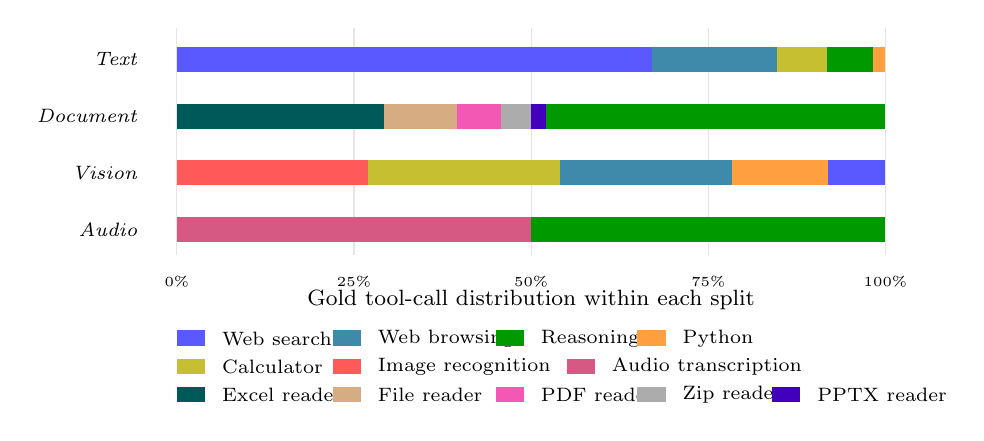
\begin{tikzpicture}[x=0.09cm,y=0.72cm]
    \foreach \x in {0,25,50,75,100} {
        \draw[gray!20] (\x,0.55) -- (\x,4.55);
        \node[font=\tiny,anchor=north] at (\x,0.35) {\x\%};
    }
    \node[font=\footnotesize] at (50,-0.25) {Gold tool-call distribution within each split};

    \node[anchor=east,font=\scriptsize] at (-4,4) {\emph{Text}};
    \fill[blue!65] (0,3.78) rectangle (67.0,4.22);
    \fill[cyan!65!black] (67.0,3.78) rectangle (84.7,4.22);
    \fill[yellow!75!black] (84.7,3.78) rectangle (91.7,4.22);
    \fill[green!60!black] (91.7,3.78) rectangle (98.3,4.22);
    \fill[orange!75] (98.3,3.78) rectangle (100,4.22);

    \node[anchor=east,font=\scriptsize] at (-4,3) {\emph{Document}};
    \fill[teal!70!black] (0,2.78) rectangle (29.2,3.22);
    \fill[brown!65] (29.2,2.78) rectangle (39.6,3.22);
    \fill[magenta!65] (39.6,2.78) rectangle (45.8,3.22);
    \fill[gray!65] (45.8,2.78) rectangle (50.0,3.22);
    \fill[purple!35!blue] (50.0,2.78) rectangle (52.1,3.22);
    \fill[green!60!black] (52.1,2.78) rectangle (100,3.22);

    \node[anchor=east,font=\scriptsize] at (-4,2) {\emph{Vision}};
    \fill[red!65] (0,1.78) rectangle (27.0,2.22);
    \fill[yellow!75!black] (27.0,1.78) rectangle (54.1,2.22);
    \fill[cyan!65!black] (54.1,1.78) rectangle (78.4,2.22);
    \fill[orange!75] (78.4,1.78) rectangle (91.9,2.22);
    \fill[blue!65] (91.9,1.78) rectangle (100,2.22);

    \node[anchor=east,font=\scriptsize] at (-4,1) {\emph{Audio}};
    \fill[purple!65] (0,0.78) rectangle (50,1.22);
    \fill[green!60!black] (50,0.78) rectangle (100,1.22);

    \fill[blue!65] (0,-1.05) rectangle (4,-0.78);
    \node[anchor=west,font=\scriptsize] at (5,-0.92) {Web search};
    \fill[cyan!65!black] (22,-1.05) rectangle (26,-0.78);
    \node[anchor=west,font=\scriptsize] at (27,-0.92) {Web browsing};
    \fill[green!60!black] (45,-1.05) rectangle (49,-0.78);
    \node[anchor=west,font=\scriptsize] at (50,-0.92) {Reasoning};
    \fill[orange!75] (65,-1.05) rectangle (69,-0.78);
    \node[anchor=west,font=\scriptsize] at (70,-0.92) {Python};

    \fill[yellow!75!black] (0,-1.55) rectangle (4,-1.28);
    \node[anchor=west,font=\scriptsize] at (5,-1.42) {Calculator};
    \fill[red!65] (22,-1.55) rectangle (26,-1.28);
    \node[anchor=west,font=\scriptsize] at (27,-1.42) {Image recognition};
    \fill[purple!65] (55,-1.55) rectangle (59,-1.28);
    \node[anchor=west,font=\scriptsize] at (60,-1.42) {Audio transcription};

    \fill[teal!70!black] (0,-2.05) rectangle (4,-1.78);
    \node[anchor=west,font=\scriptsize] at (5,-1.92) {Excel reader};
    \fill[brown!65] (22,-2.05) rectangle (26,-1.78);
    \node[anchor=west,font=\scriptsize] at (27,-1.92) {File reader};
    \fill[magenta!65] (45,-2.05) rectangle (49,-1.78);
    \node[anchor=west,font=\scriptsize] at (50,-1.92) {PDF reader};
    \fill[gray!65] (65,-2.05) rectangle (69,-1.78);
    \node[anchor=west,font=\scriptsize] at (70,-1.92) {Zip reader};
    \fill[purple!35!blue] (84,-2.05) rectangle (88,-1.78);
    \node[anchor=west,font=\scriptsize] at (89,-1.92) {PPTX reader};
\end{tikzpicture}}
\caption{Within-split gold tool-slot distribution across the 165-task GAIA set. Bars are normalized within each split and show relative tool composition rather than raw counts. In \emph{Document}, attachment-access calls are displayed as typed document-reader calls: 29.2\% spreadsheet reader, 10.4\% generic file reader, 6.3\% PDF reader, 4.2\% archive reader, and 2.1\% presentation reader.}
\label{fig:appendix-gaia-tool-distribution}
\end{figure}

The split-level profile is intentionally skewed. \emph{Text} is search-heavy, \emph{Document} concentrates on typed attachment access plus reasoning, \emph{Vision} combines image recognition with calculation, browsing, and code execution, and \emph{Audio} pairs transcription with downstream reasoning.

\begin{table}[H]
\centering
\scriptsize
\setlength{\tabcolsep}{5pt}
%\resizebox{\linewidth}{!}{%
\begin{tabular}{lp{0.48\linewidth}p{0.32\linewidth}}
\toprule
Domain & Main tool families used by the gold references & Role in the benchmark \\
\midrule
\emph{Text} & web search, web browsing, calculator, reasoning, Python execution & Search and inspect sources, then compute intermediate quantities. \\
\emph{Document} & spreadsheet reader, generic file reader, PDF reader, archive extractor, presentation reader, reasoning & Parse local attachments and combine document evidence with reasoning. \\
\emph{Vision} & image recognition, calculator, web browsing, Python execution, web search & Convert visual evidence into textual or structured observations before computing or inspecting supporting sources. \\
\emph{Audio} & audio transcription, reasoning & Transcribe audio evidence and solve text constraints over the transcript. \\
\bottomrule
\end{tabular}
%}
\vspace{0.05cm}
\caption{Domain-level tool demand under the shared 16-tool executable catalog. All English GAIA tasks see the same 16 prompt-visible tools; domain-specific demand is reflected in task attachments and gold tool references rather than in a different visible tool list.}
\label{tab:appendix-domain-tool-interface}
\end{table}

\FloatBarrier

\section{Augmented GAIA Data Profile}
\label{sec:appendix-data-profile}

\subsection{Dataset Views and Accounting}
\label{subsec:appendix-data-accounting}

Augmented GAIA keeps the original 165 GAIA tasks, queries, attachments, and final-answer targets unchanged. The release adds three evaluation-facing layers: a tool-reference layer for grounded tool scoring, \model{GPT-4o} dependency annotations for planning-reference construction, and a Gemma 4 behavior-preserving replay-filtered async-ordering view used as the Augmented GAIA reference ordering layer. 
The unfiltered dependency view contains the task-level DAGs together with all candidate dependency-preserving orderings derived from them. The filtered ordering view keeps the same task-level dependency DAGs but retains only behavior-preserving async orderings under the Gemma 4 replay policy. The native chain remains available for every task, so tasks with no retained async ordering fall back to the original chain reference rather than being removed from the benchmark.

\begin{table}[H]
\centering
\scriptsize
\setlength{\tabcolsep}{3pt}
\begin{tabular}{l r p{0.55\linewidth}}
\toprule
Quantity & Value & Interpretation \\
\midrule
Tasks & 165 & Original GAIA task instances retained without changing query, attachment, or answer target. \\
Planning nodes & 1{,}284 & Step inventory in the \model{GPT-4o} dependency DAG annotations. \\
Dependency edges & 1{,}086 & Reduced dependency edges used by the planning-reference layer. \\
Candidate async orderings & 1{,}771 & Candidate dependency-preserving non-native orderings generated from the unfiltered dependency view. \\
Retained async orderings & 1{,}357 & Gemma 4 behavior-preserving non-native orderings retained in the filtered ordering view. \\
Native-only tasks & 107 & Tasks with no retained async ordering; the native chain remains the sole reference. \\
Tasks with $\geq 1$ retained async ordering & 58 (35.2\%) & Tasks with at least one retained reference beyond the native chain. \\
Tasks with exactly 1 retained async ordering & 4 (2.4\%) & Native chain plus one retained async reference. \\
Tasks with $\geq 2$ retained async orderings & 54 (32.7\%) & Multi-order-rich subset used for flexible-order stress tests. \\
Mean native steps per task & 7.78 & Average size of the original step inventory. \\
Mean dependency edges per task & 6.58 & Average reduced dependency-edge count. \\
\bottomrule
\end{tabular}
%}
\vspace{0.01cm}
\caption{DAG and paper-accounting summary computed directly from the final Augmented GAIA release files.}
\label{tab:appendix-augmented-gaia-accounting}
\end{table}

\subsection{Replay-Filtered Coverage}
\label{subsec:appendix-data-coverage}

\begin{figure}[H]
\centering
\resizebox{0.80\linewidth}{!}{%
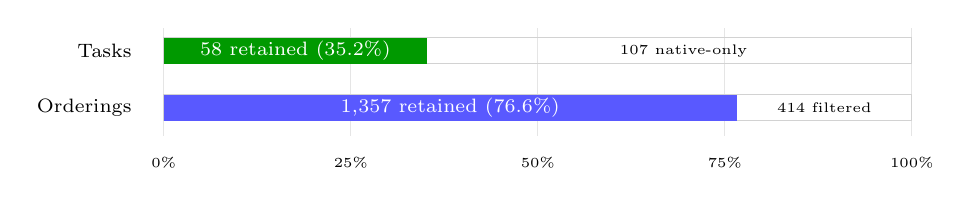
\begin{tikzpicture}[x=0.095cm,y=0.72cm]
    \foreach \x in {0,25,50,75,100} {
        \draw[gray!20] (\x,0.55) -- (\x,2.45);
        \node[font=\tiny,anchor=north] at (\x,0.35) {\x\%};
    }
    \node[anchor=east,font=\scriptsize] at (-3,2.05) {Tasks};
    \draw[gray!35] (0,1.82) rectangle (100,2.28);
    \fill[green!60!black] (0,1.82) rectangle (35.2,2.28);
    \node[font=\scriptsize,text=white] at (17.6,2.05) {$58$ retained (35.2\%)};
    \node[font=\tiny] at (69.5,2.05) {$107$ native-only};

    \node[anchor=east,font=\scriptsize] at (-3,1.05) {Orderings};
    \draw[gray!35] (0,0.82) rectangle (100,1.28);
    \fill[blue!65] (0,0.82) rectangle (76.6,1.28);
    \node[font=\scriptsize,text=white] at (38.3,1.05) {$1{,}357$ retained (76.6\%)};
    \node[font=\tiny] at (88.3,1.05) {$414$ filtered};
\end{tikzpicture}}
\caption{Replay-filtered Augmented GAIA coverage. The task bar shows the share of tasks with at least one retained async ordering beyond the native chain; the ordering bar shows the Gemma 4 behavior-preserving retention rate over candidate async orderings.}
\label{fig:appendix-augmented-gaia-coverage}
\end{figure}

\begin{figure}[H]
\centering
\resizebox{\linewidth}{!}{%
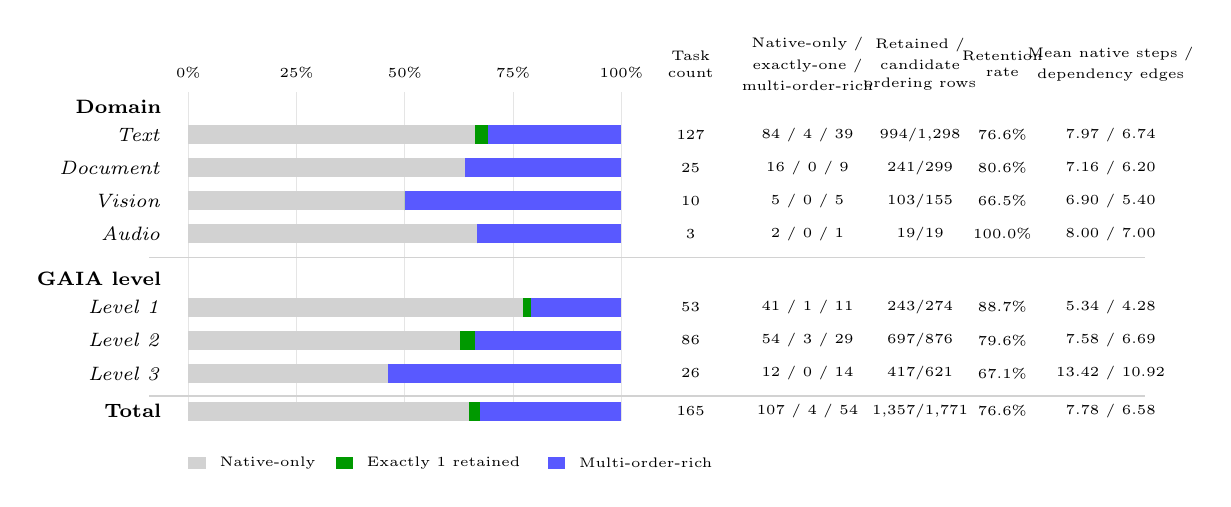
\begin{tikzpicture}[x=0.055cm,y=0.60cm]
    \foreach \x in {0,25,50,75,100} {
        \draw[gray!20] (\x,1.70) -- (\x,8.65);
        \node[font=\tiny,anchor=south] at (\x,8.73) {\x\%};
    }

    \node[font=\tiny] at (116,9.25) {\shortstack{Task\\count}};
    \node[font=\tiny] at (143,9.25) {\shortstack{Native-only /\\exactly-one /\\multi-order-rich}};
    \node[font=\tiny] at (169,9.25) {\shortstack{Retained /\\candidate\\ordering rows}};
    \node[font=\tiny] at (188,9.25) {\shortstack{Retention\\rate}};
    \node[font=\tiny] at (213,9.25) {\shortstack{Mean native steps /\\dependency edges}};

    \node[anchor=east,font=\scriptsize\bfseries] at (-4,8.35) {Domain};
	    \node[anchor=east,font=\scriptsize] at (-4,7.75) {\emph{Text}};
	    \fill[gray!35] (0,7.55) rectangle (66.1,7.95);
	    \fill[green!60!black] (66.1,7.55) rectangle (69.3,7.95);
	    \fill[blue!65] (69.3,7.55) rectangle (100,7.95);
    \node[font=\tiny] at (116,7.75) {127};
    \node[font=\tiny] at (143,7.75) {84 / 4 / 39};
    \node[font=\tiny] at (169,7.75) {994/1{,}298};
    \node[font=\tiny] at (188,7.75) {76.6\%};
    \node[font=\tiny] at (213,7.75) {7.97 / 6.74};

	    \node[anchor=east,font=\scriptsize] at (-4,7.05) {\emph{Document}};
	    \fill[gray!35] (0,6.85) rectangle (64.0,7.25);
	    \fill[green!60!black] (64.0,6.85) rectangle (64.0,7.25);
	    \fill[blue!65] (64.0,6.85) rectangle (100,7.25);
    \node[font=\tiny] at (116,7.05) {25};
    \node[font=\tiny] at (143,7.05) {16 / 0 / 9};
    \node[font=\tiny] at (169,7.05) {241/299};
    \node[font=\tiny] at (188,7.05) {80.6\%};
    \node[font=\tiny] at (213,7.05) {7.16 / 6.20};

	    \node[anchor=east,font=\scriptsize] at (-4,6.35) {\emph{Vision}};
	    \fill[gray!35] (0,6.15) rectangle (50.0,6.55);
	    \fill[green!60!black] (50.0,6.15) rectangle (50.0,6.55);
	    \fill[blue!65] (50.0,6.15) rectangle (100,6.55);
    \node[font=\tiny] at (116,6.35) {10};
    \node[font=\tiny] at (143,6.35) {5 / 0 / 5};
    \node[font=\tiny] at (169,6.35) {103/155};
    \node[font=\tiny] at (188,6.35) {66.5\%};
    \node[font=\tiny] at (213,6.35) {6.90 / 5.40};

	    \node[anchor=east,font=\scriptsize] at (-4,5.65) {\emph{Audio}};
	    \fill[gray!35] (0,5.45) rectangle (66.7,5.85);
	    \fill[green!60!black] (66.7,5.45) rectangle (66.7,5.85);
	    \fill[blue!65] (66.7,5.45) rectangle (100,5.85);
    \node[font=\tiny] at (116,5.65) {3};
    \node[font=\tiny] at (143,5.65) {2 / 0 / 1};
    \node[font=\tiny] at (169,5.65) {19/19};
    \node[font=\tiny] at (188,5.65) {100.0\%};
    \node[font=\tiny] at (213,5.65) {8.00 / 7.00};

    \draw[gray!35] (-9,5.15) -- (221,5.15);
    \node[anchor=east,font=\scriptsize\bfseries] at (-4,4.70) {GAIA level};
	    \node[anchor=east,font=\scriptsize] at (-4,4.10) {\emph{Level 1}};
	    \fill[gray!35] (0,3.90) rectangle (77.4,4.30);
	    \fill[green!60!black] (77.4,3.90) rectangle (79.2,4.30);
	    \fill[blue!65] (79.2,3.90) rectangle (100,4.30);
    \node[font=\tiny] at (116,4.10) {53};
    \node[font=\tiny] at (143,4.10) {41 / 1 / 11};
    \node[font=\tiny] at (169,4.10) {243/274};
    \node[font=\tiny] at (188,4.10) {88.7\%};
    \node[font=\tiny] at (213,4.10) {5.34 / 4.28};

	    \node[anchor=east,font=\scriptsize] at (-4,3.40) {\emph{Level 2}};
	    \fill[gray!35] (0,3.20) rectangle (62.8,3.60);
	    \fill[green!60!black] (62.8,3.20) rectangle (66.3,3.60);
	    \fill[blue!65] (66.3,3.20) rectangle (100,3.60);
    \node[font=\tiny] at (116,3.40) {86};
    \node[font=\tiny] at (143,3.40) {54 / 3 / 29};
    \node[font=\tiny] at (169,3.40) {697/876};
    \node[font=\tiny] at (188,3.40) {79.6\%};
    \node[font=\tiny] at (213,3.40) {7.58 / 6.69};

	    \node[anchor=east,font=\scriptsize] at (-4,2.70) {\emph{Level 3}};
	    \fill[gray!35] (0,2.50) rectangle (46.2,2.90);
	    \fill[green!60!black] (46.2,2.50) rectangle (46.2,2.90);
	    \fill[blue!65] (46.2,2.50) rectangle (100,2.90);
    \node[font=\tiny] at (116,2.70) {26};
    \node[font=\tiny] at (143,2.70) {12 / 0 / 14};
    \node[font=\tiny] at (169,2.70) {417/621};
    \node[font=\tiny] at (188,2.70) {67.1\%};
    \node[font=\tiny] at (213,2.70) {13.42 / 10.92};

    \draw[gray!35] (-9,2.22) -- (221,2.22);
	    \node[anchor=east,font=\scriptsize\bfseries] at (-4,1.90) {Total};
	    \fill[gray!35] (0,1.70) rectangle (64.8,2.10);
	    \fill[green!60!black] (64.8,1.70) rectangle (67.3,2.10);
	    \fill[blue!65] (67.3,1.70) rectangle (100,2.10);
    \node[font=\tiny] at (116,1.90) {165};
    \node[font=\tiny] at (143,1.90) {107 / 4 / 54};
    \node[font=\tiny] at (169,1.90) {1{,}357/1{,}771};
    \node[font=\tiny] at (188,1.90) {76.6\%};
    \node[font=\tiny] at (213,1.90) {7.78 / 6.58};

	    \fill[gray!35] (0,0.68) rectangle (4,0.92);
	    \node[anchor=west,font=\tiny] at (5,0.80) {Native-only};
	    \fill[green!60!black] (34,0.68) rectangle (38,0.92);
	    \node[anchor=west,font=\tiny] at (39,0.80) {Exactly 1 retained};
	    \fill[blue!65] (83,0.68) rectangle (87,0.92);
	    \node[anchor=west,font=\tiny] at (88,0.80) {Multi-order-rich};
\end{tikzpicture}}
\caption{Augmented GAIA construction profile by input domain and GAIA level. Stacked bars decompose each slice's tasks into native-only, exactly-one-retained, and multi-order-rich cases; the right columns report task counts, retained candidate-ordering rows, retention rate, and mean native steps/dependency edges per task, with the final row giving the full-release total.}
\label{fig:appendix-augmented-gaia-construction-profile}
\end{figure}

This profile separates three notions that are easy to conflate. First, the dependency DAG is task-level structure: all 165 tasks receive a \model{GPT-4o} dependency DAG over the original planning-intent steps. Second, candidate async orderings are construction-time realizations sampled from those DAGs; they are not new tasks and do not change the answer target. Third, Gemma 4 replay filtering selects the ordering rows that preserve native-chain execution behavior under the shared tool layer. The result is a conservative augmentation: 107 tasks remain native-chain only, 4 tasks add exactly one retained async reference, and 54 tasks form the multi-order-rich subset used for the strongest flexible-order diagnostics.

\subsection{Reference-Validated Critical Path vs. Native Chain Length}
\label{subsec:appendix-critical-path-profile}

To check whether the final Augmented GAIA reference set exposes meaningful
parallelism, we summarize the replay-filtered reference orderings rather than
unfiltered dependency annotations. For each task $q$, let $L_q$ be the native
chain length. We induce a conservative partial order from the final Augmented
GAIA references by keeping an ordering constraint only when it appears in every
retained reference ordering for that task; let $C_q$ be the longest path length
in this reference-validated partial order. We define the parallelism ratio as
\[
  \rho_q = 1 - \frac{C_q}{L_q}.
\]
A value of $\rho_q=0$ means the final references preserve the native chain
order, while larger values indicate replay-validated reordering structure.
Normalized Kendall distance is row-level and measures how far each retained
reference ordering moves from the native chain. Figure~\ref{fig:appendix-critical-path-buckets}
first summarizes the three replay-filtered coverage buckets, and
Table~\ref{tab:appendix-critical-path} reports the same diagnostic over
increasingly strict retained-ordering thresholds. The $\geq 2$ threshold is the
multi-order-rich subset used in the main flexible-order diagnostics.

\begin{figure}[H]
\centering
\resizebox{0.76\linewidth}{!}{%
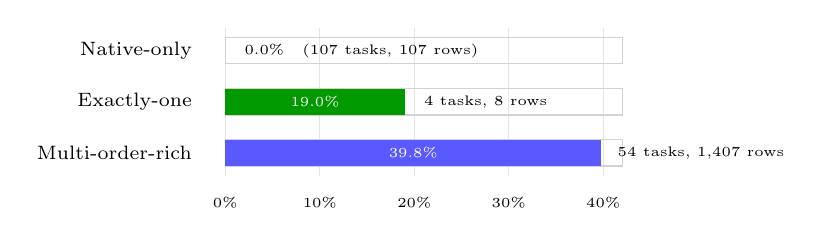
\begin{tikzpicture}[x=0.12cm,y=0.72cm]
    \foreach \x in {0,10,20,30,40} {
        \draw[gray!20] (\x,0.55) -- (\x,3.15);
        \node[font=\tiny,anchor=north] at (\x,0.35) {\x\%};
    }
    \node[anchor=east,font=\scriptsize] at (-2.5,2.75) {Native-only};
    \draw[gray!35] (0,2.52) rectangle (42,2.98);
    \node[anchor=west,font=\tiny] at (1.0,2.75) {0.0\% \; (107 tasks, 107 rows)};

    \node[anchor=east,font=\scriptsize] at (-2.5,1.85) {Exactly-one};
    \draw[gray!35] (0,1.62) rectangle (42,2.08);
    \fill[green!60!black] (0,1.62) rectangle (19.0,2.08);
    \node[font=\tiny,text=white] at (9.5,1.85) {19.0\%};
    \node[anchor=west,font=\tiny] at (20.0,1.85) {4 tasks, 8 rows};

    \node[anchor=east,font=\scriptsize] at (-2.5,0.95) {Multi-order-rich};
    \draw[gray!35] (0,0.72) rectangle (42,1.18);
    \fill[blue!65] (0,0.72) rectangle (39.8,1.18);
    \node[font=\tiny,text=white] at (19.9,0.95) {39.8\%};
    \node[anchor=west,font=\tiny] at (40.5,0.95) {54 tasks, 1{,}407 rows};
\end{tikzpicture}}
\caption{Reference-validated parallelism by replay-filtered coverage bucket. Rows count final Augmented GAIA references: native-only tasks contribute one native row, exactly-one tasks contribute one native plus one retained non-native row, and multi-order-rich tasks contribute one native plus at least two retained non-native rows.}
\label{fig:appendix-critical-path-buckets}
\end{figure}

\begin{table}[H]
\centering
\scriptsize
\setlength{\tabcolsep}{3.2pt}
\makebox[\linewidth][c]{%
\begin{tabular}{l r r c c}
\toprule
Threshold & Tasks & \shortstack{Retained\\rows} & \shortstack{Parallelism\\mean / med.} & \shortstack{Kendall dist.\\mean / med. / max} \\
\midrule
$\geq 1$ & 58 & 1{,}357 & 40.0\% / 40.0\% & 0.230 / 0.200 / 0.667 \\
$\geq 2$ (multi-order-rich) & 54 & 1{,}353 & 40.1\% / 40.0\% & 0.230 / 0.200 / 0.667 \\
$\geq 5$ & 40 & 1{,}314 & 40.4\% / 40.0\% & 0.232 / 0.205 / 0.667 \\
$\geq 10$ & 32 & 1{,}266 & 41.0\% / 40.0\% & 0.236 / 0.209 / 0.667 \\
$\geq 20$ & 26 & 1{,}163 & 42.2\% / 42.9\% & 0.246 / 0.222 / 0.667 \\
$\geq 50$ & 13 & 650 & 42.6\% / 40.0\% & 0.259 / 0.222 / 0.667 \\
\bottomrule
\end{tabular}
}
\vspace{0.05cm}
\caption{Reference-validated critical-path and reordering diagnostic over Gemma 4-retained non-native async-ordering thresholds. Parallelism is computed from the final Augmented GAIA reference orderings; Kendall distance is computed between each retained reference ordering and the native chain.}
\label{tab:appendix-critical-path}
\end{table}

\FloatBarrier
\clearpage
\section{Qualitative multi-order example: Native GAIA chain vs. Augmented GAIA DAG}
\label{sec:appendix-qualitative-multi-order}

\begin{figure}[H]
\centering
\makebox[\textwidth][c]{%
\includegraphics[width=1\textwidth]{generated/custom_figures/qualitative_multi_order_core.png}}
\caption{Qualitative multi-order example from a Document task. The native chain serializes the two accommodation-type computations, while the augmented DAG exposes them as independent branches before the final comparison.}
\label{fig:appendix-qualitative-multi-order}
\end{figure}

This example illustrates the kind of planning behavior that the augmented
reference is intended to credit. The task asks the model to compare the average
ratings of two accommodation types in an attached PDF. The native chain is a
valid execution: open the PDF, compute the hotel total and mean, then compute
the rental-house total and mean, and finally compare the two averages. However,
the ordering between the hotel branch and the rental-house branch is incidental
to the solution. Once the PDF has been read, the two branch-level summaries can
be computed independently before the final comparison.

The augmented dependency DAG preserves the same step inventory and answer target
but removes the requirement that the hotel branch must precede the rental-house
branch. Both branches remain dependent on opening the PDF, and the final compare
node depends on both branch means. Thus, the augmented reference does not change
the task or invent an alternative solution; it exposes the partial order that is
already implicit in the native solution. This is the distinction that
\metric{EdgeF1} is meant to measure: whether the predicted planning graph
recovers necessary dependencies rather than the arbitrary serialization of one
recorded execution.

The model plan on the right captures the same planning intent. The raw emitted
abstract plan extracts the accommodations and ratings, groups them by type,
computes the average rating for each accommodation type, and compares the
averages. In the figure, the average-computation node is expanded into hotel and
rental-house mean branches to make the recoverable dependency fork explicit.
Under the native sequential chain, this intent can be penalized because it does
not reproduce the hotel-then-rental order exactly. Under Augmented GAIA, the same
plan receives credit because it respects the dependency DAG: evidence extraction
precedes grouping, the two means are independent given the grouping, and the
answer depends on their comparison. In this instance, the model is
\model{Llama-3.1 405B}; its native \metric{PlanningScore} is 0.525, while its
augmented \metric{PlanningScore} is 0.622, with paper \metric{EdgeF1} increasing
from 0.250 to 0.444 (+0.194 absolute, +77.8\% relative using the unrounded
scores) and the final stage matching the gold answer
\emph{Hotels}.

\FloatBarrier
\clearpage


\section{Behavior-Preserving Replay Filter for Augmented GAIA Reference Construction}
\label{sec:appendix-replay-filter-current}

The async ordering layer of Augmented GAIA is filtered by a behavior-preserving replay procedure under \model{Gemma 4} as the replay model. The filter operationalizes plan equivalence through outcome reproduction (Section~\ref{sec:dataset-validation}): a candidate ordering is retained when its reordered replay reproduces the native chain's final-answer outcome on the same task under the shared executable tool layer, and is otherwise filtered out. This frames augmentation as a conservative extension of the native chain rather than as a filter that selects only rows solved correctly by a strong model.

Outcome reproduction is operationalized as gold-evaluator equivalence on the answer string. Two replays reproduce the same outcome in either of two cases: (i) both replays produce gold-equivalent correct answers, possibly with surface-form differences (numeric formatting such as $1$ vs. $1.0$, accepted aliases such as St. Petersburg vs. Saint Petersburg, or tolerance-equivalent numbers such as $563.9$ vs. $564.0$); or (ii) both replays produce the same wrong answer. Orderings whose reordered replay yields a different outcome than the native chain---changing a correct answer to a wrong one, recovering a correct answer where the native chain failed, or producing a different wrong answer---are filtered. Retaining the same-wrong category is the conservative choice for plan equivalence: when the native and reordered replays converge to the same incorrect outcome, the reordering has not altered the executable behavior of the native plan, even if that behavior happens to be incorrect on the gold target. The filter does not select for orderings that improve solvability.

Table~\ref{tab:appendix-current-replay-filter} summarizes the filter result. Of $1{,}771$ candidate async orderings, $1{,}357$ ($76.6\%$) are retained and $414$ ($23.4\%$) are filtered. Among the $414$ filtered orderings, $88$ ($21.3\%$ of filtered) have no usable native-chain replay output, so the row is not treated as an augmentation-specific failure: the native chain itself does not produce a definite outcome to reproduce. The remaining $326$ ($78.7\%$ of filtered) correspond to ordering-specific non-reproduction, where the native chain produces an outcome but the reordered replay produces a different one.

\begin{table}[H]
\centering
\scriptsize
\setlength{\tabcolsep}{10pt}
\begin{tabular}{lrr}
\toprule
Item & Count & Rate \\
\midrule
Total candidate ordering rows & 1{,}771 & 100.0\% (1{,}771/1{,}771) \\
Retained under behavior-preserving filter & 1{,}357 & 76.6\% (1{,}357/1{,}771) \\
Filtered under behavior-preserving filter & 414 & 23.4\% (414/1{,}771) \\
\midrule
Native chain replay unavailable & 88 & 21.3\% of filtered (88/414) \\
Ordering-specific non-reproducible outcome & 326 & 78.7\% of filtered (326/414) \\
\bottomrule
\end{tabular}
\vspace{0.05cm}
\caption{\model{Gemma 4} behavior-preserving replay filter summary for Augmented GAIA reference construction.}
\label{tab:appendix-current-replay-filter}
\end{table}

Table~\ref{tab:appendix-current-replay-outcomes} reports the full outcome typology for all $1{,}771$ candidate orderings. The first three rows are retained under the behavior-preserving policy ($1{,}219$ both-correct text-equivalent, $37$ both-correct surface-different, and $101$ both-wrong same-answer); the remaining five rows are filtered. The two largest filtered categories are \emph{both wrong, different wrong answers} ($151$, $8.5\%$ of all candidates) and \emph{native correct, reordered wrong} ($69$, $3.9\%$). The latter is the augmentation-specific failure mode where reordering an originally correct execution produces a wrong outcome under \model{Gemma 4}; the former represents executions that fail in different ways under reordering, indicating that the reordered trajectory diverges from the native one.

\begin{table}[H]
\centering
\scriptsize
\begin{tabular}{lrr}
\toprule
Replay outcome & Count & Rate \\
\midrule
Native and reordered answers both correct and text-equivalent & 1{,}219 & 68.8\% (1{,}219/1{,}771) \\
Native and reordered answers both correct but surface-different & 37 & 2.1\% (37/1{,}771) \\
Both answers wrong, same wrong answer & 101 & 5.7\% (101/1{,}771) \\
Both answers wrong, different wrong answers & 151 & 8.5\% (151/1{,}771) \\
Native correct, reordered wrong & 69 & 3.9\% (69/1{,}771) \\
Native wrong, reordered correct & 68 & 3.8\% (68/1{,}771) \\
Native chain replay produced no usable answer & 88 & 5.0\% (88/1{,}771) \\
Reordered replay produced no usable answer & 38 & 2.1\% (38/1{,}771) \\
\bottomrule
\end{tabular}
\vspace{0.05cm}
\caption{\model{Gemma 4} replay outcome typology over all $1{,}771$ candidate async orderings. Rows 1--3 are retained under the behavior-preserving filter; rows 4--8 are filtered.}
\label{tab:appendix-current-replay-outcomes}
\end{table}

Two design points are worth noting for reproducibility. First, the filter operationalizes plan equivalence through outcome reproduction under a single replay model, so the retention pool reflects \model{Gemma 4}'s execution profile in particular; an alternative multi-model agreement filter would yield a smaller pool with stronger cross-model behavior alignment, at the cost of further reducing the retained orderings beyond the present $1{,}357$. Second, retaining \emph{both wrong, same wrong answer} rows is a deliberate conservatism: these orderings preserve native-chain executable behavior under reordering, even though the underlying behavior is itself incorrect on the gold target, and excluding them would convert the filter into a correctness-conditional selector rather than a behavior-preservation filter. Section~\ref{sec:limitations} discusses the implications of these design choices for the scope of the augmentation effect we report.


\section{Human Dependency Spot Check}
\label{sec:appendix-spot-check-current}

To assess the semantic quality of the synthesized dependency graphs, we conduct
an independent human spot check over \(30\) tasks. The sampled tasks are selected
from instances with multiple admissible execution orders, where dependency
quality is especially consequential: a spurious edge can unnecessarily constrain
the execution graph, while a missing edge can admit invalid reorderings.

Three independent annotators review each sampled task. For each task, annotators
are given the original query, the chain-style step descriptions, the synthesized
dependency edges, and a sampled set of step pairs for which no edge was asserted.
Annotators are instructed to judge dependencies using only the provided query and
step sequence, without external search or additional task execution. This design
isolates whether the dependency relation is supported by the annotated executable
plan itself.

The annotation form contains two row types. For \emph{asserted edges},
annotators judge whether the proposed parent--child dependency actually exists.
An asserted edge is judged correct if the parent step provides information,
state, context, or an intermediate result required for the child step to be
validly executed. These rows estimate the false-positive rate of the synthesized
dependency graph. For \emph{sampled nonedges}, annotators judge whether the
absence of an edge is correct or whether a necessary dependency was missed.
These rows estimate false negatives among sampled unasserted step pairs. A
separate free-form field allows annotators to record additional missing
dependencies outside the sampled nonedge rows.

The completed forms contain \(351\) judgments per annotator: \(248\) asserted
edges and \(103\) sampled nonedges. Pooling both row types as binary
dependency-existence judgments, annotators are unanimous on \(330/351\) rows
(\(94.0\%\)), with Fleiss \(\kappa=0.905\). Pairwise Cohen \(\kappa\) values are
\(0.959\), \(0.885\), and \(0.872\). This high pooled agreement indicates that
the binary distinction between dependency and non-dependency is stable under
independent human review.

For asserted edges, majority vote judges \(244/248\) edges correct
(\(98.4\%\)) and \(4/248\) incorrect (\(1.6\%\)). Annotators are unanimous on
\(232/248\) asserted edges (\(93.5\%\)). Fleiss \(\kappa\) for asserted-edge
correctness is \(0.363\), with pairwise Cohen \(\kappa\) values of \(0.605\),
\(0.293\), and \(0.274\). This lower chance-corrected agreement should be
interpreted together with the strong prevalence imbalance in this subset:
because nearly all asserted edges are judged correct, the expected chance
agreement is high, compressing \(\kappa\) despite high raw agreement.

For sampled nonedges, majority vote judges \(96/103\) pairs as correctly having
no dependency (\(93.2\%\)) and \(7/103\) as missed dependencies (\(6.8\%\)).
Annotators are unanimous on \(98/103\) sampled nonedges (\(95.1\%\)). Fleiss
\(\kappa\) is \(0.755\), with pairwise Cohen \(\kappa\) values of \(0.928\),
\(0.693\), and \(0.641\). The free-form fields identify \(10\) unique additional
missing dependencies; \(8\) receive two-annotator support, while \(2\) receive
single-annotator support.

Overall, the spot check indicates that the synthesized dependency graphs have
high precision on asserted edges and limited false negatives among sampled
nonedges. The remaining errors are concentrated in a small number of omitted
dependencies rather than widespread spurious dependencies. These results support
the use of the synthesized graphs as binary dependency references for
order-aware planning evaluation.

\FloatBarrier
\section{Cross-Benchmark Scope}
\label{sec:appendix-cross-benchmark}

We use TaskBench and UltraTool to test whether the end-to-end evaluation
machinery transfers to public benchmarks beyond our GAIA-derived setting.
\emph{Augmented GAIA} is the benchmark instantiation in this study that fits the
full three-facet framework: native GAIA supplies verifiable final-answer targets,
while our annotations add the explicit tool layer and dependency-aware planning
references needed for planning and tool-use evaluation.

TaskBench and UltraTool are used as subsampled cross-benchmark checks with the
same seven-model pool used in the main GAIA tables. For TaskBench, we construct
a balanced 1{,}000-example subset with 500 DAG-style examples and 500
chain-style examples. For UltraTool, we use a 1{,}000-example English subset.
To fit these datasets into our staged evaluation framework, we normalize their
original records into a shared evaluation format, including task records,
planning references, tool-reference fields, and model-facing input templates.
These format adjustments are used only to make the benchmarks compatible with
our evaluation pipeline and do not change the underlying task intent.

Both datasets support the planning and tool-use facets, but they lack the
human-auditable final-answer target used for the Accepted Answer rate.
Facet C is therefore intentionally left blank for these benchmarks. Their role
is to test whether the planning/tool evaluation machinery transfers beyond
Augmented GAIA, rather than to extend final-answer evaluation.

\begin{table}[t]
\centering
\scriptsize
\setlength{\tabcolsep}{0.6pt}
%\resizebox{\linewidth}{!}{%
\makebox[\linewidth][c]{%
\begin{tabular}{llcccccccccc}
\toprule
\multirow{3}{*}{Model} & \multirow{3}{*}{Params}
& \multicolumn{3}{c}{(A) Plan Structural Fidelity}
& \multicolumn{3}{c}{(B) Tool Invocation Accuracy}
& \multicolumn{4}{c}{(C) End-Task Answer Correctness} \\
\cmidrule(lr){3-5}\cmidrule(lr){6-8}\cmidrule(lr){9-12}
& & \metric{NodeF1} & \metric{EdgeF1} & \metric{PlanningScore}
& \metric{ToolF1} & \metric{ParamF1} & \metric{ParamValueF1}
& EM & \metric{TokenF1} & Raw rate & Accepted rate \\
\midrule
\multicolumn{12}{@{}l}{\textbf{TaskBench}} \\
\model{Mistral Large 3} & 675B & 0.668 & 0.235 & 0.451 & 0.659 & 0.457 & 0.266 & -- & -- & -- & -- \\
\model{Llama-3.1} & 405B & 0.771 & 0.367 & 0.569 & 0.767 & 0.600 & 0.393 & -- & -- & -- & -- \\
\model{Llama-3.3} & 70B & 0.705 & 0.337 & 0.521 & 0.725 & 0.537 & 0.341 & -- & -- & -- & -- \\
\model{Gemma 4} & 31B & 0.839 & 0.439 & 0.639 & 0.822 & 0.655 & 0.453 & -- & -- & -- & -- \\
\model{Mistral Small 3.2} & 24B & 0.792 & 0.398 & 0.595 & 0.751 & 0.596 & 0.387 & -- & -- & -- & -- \\
\model{Llama-4 Maverick} & 17B & 0.812 & 0.436 & 0.624 & 0.774 & 0.610 & 0.406 & -- & -- & -- & -- \\
\model{Gemma 3} & 12B & 0.723 & 0.318 & 0.521 & 0.708 & 0.525 & 0.331 & -- & -- & -- & -- \\
\emph{Model mean} & -- & 0.759 & 0.361 & 0.560 & 0.744 & 0.569 & 0.368 & -- & -- & -- & -- \\
\midrule
\multicolumn{12}{@{}l}{\textbf{UltraTool}} \\
\model{Mistral Large 3} & 675B & 0.492 & 0.079 & 0.286 & 0.866 & 0.630 & 0.395 & -- & -- & -- & -- \\
\model{Llama-3.1} & 405B & 0.517 & 0.105 & 0.311 & 0.932 & 0.682 & 0.380 & -- & -- & -- & -- \\
\model{Llama-3.3} & 70B & 0.492 & 0.103 & 0.298 & 0.740 & 0.518 & 0.312 & -- & -- & -- & -- \\
\model{Gemma 4} & 31B & 0.558 & 0.116 & 0.337 & 0.943 & 0.795 & 0.549 & -- & -- & -- & -- \\
\model{Mistral Small 3.2} & 24B & 0.524 & 0.107 & 0.315 & 0.916 & 0.670 & 0.412 & -- & -- & -- & -- \\
\model{Llama-4 Maverick} & 17B & 0.518 & 0.120 & 0.319 & 0.955 & 0.709 & 0.445 & -- & -- & -- & -- \\
\model{Gemma 3} & 12B & 0.516 & 0.107 & 0.312 & 0.850 & 0.622 & 0.366 & -- & -- & -- & -- \\
\emph{Model mean} & -- & 0.517 & 0.105 & 0.311 & 0.886 & 0.661 & 0.408 & -- & -- & -- & -- \\
\bottomrule
\end{tabular}
}
%}
\vspace{0.005cm}
\caption{Cross-benchmark results on TaskBench and UltraTool. Facet C is blank because neither dataset provides verifiable final-answer targets.}
\label{tab:appendix-cross-benchmark-taskbench-ultratool}
\end{table}
\FloatBarrier
\section{Tool-clean Variants}
\label{sec:appendix-tool-clean}

\subsection{Tool-Clean Filtering Rules}
A prediction is \emph{tool-clean} when it has no parse error, ATS $\ge 0.5$, and TISR $\ge 0.7$. ATS is a gold-slot coverage measure: it asks how many required gold tool slots are matched by successful non-submit predicted tool calls. TISR is an execution-stability measure: it asks what fraction of the model's non-submit tool calls completed without runtime failure. The two quantities are complementary: a model can execute many calls successfully while still missing the gold tool slots, or it can invoke a relevant tool but fail because the argument or runtime environment is invalid.

The main planning--answer correlation diagnostic uses the GAIA Level 2 \emph{Text}/\emph{Document}/\emph{Audio} slice. Level 1 tasks are often too short for planning variation to be visible, Level 3 tasks are answer-sparse, and \emph{Vision} has too few tasks for stable per-model correlation estimates. Table~\ref{tab:tool-density-definition} summarizes the main tool-clean slice and the corresponding tool-intensive variant.

\begin{table}[H]
\centering
\scriptsize
\setlength{\tabcolsep}{5.5pt}
%\resizebox{\linewidth}{!}{%
\begin{tabular}{lcccccc}
\toprule
Slice & Extra filter & N & Accepted rate & Mean $r_{\mathrm{native}}$ & Mean $r_{\mathrm{aug}}$ & Mean $\Delta r$ \\
\midrule
Level 2 \emph{Text}/\emph{Document}/\emph{Audio} tool-clean & None & 398 & 0.201 & 0.050 & 0.065 & +0.014 \\
Tool-intensive variant & Gold tool slots $\geq 2$ & 335 & 0.212 & 0.070 & 0.086 & +0.016 \\
\bottomrule
\end{tabular}
%}
\vspace{0.05cm}
\caption{Main correlation slice and tool-intensive variant. Tool-intensive means tool-clean plus at least two gold tool slots. Mean $\Delta r$ is averaged over per-model deltas, so it can differ slightly from subtracting the rounded mean-correlation columns.}
\label{tab:tool-density-definition}
\end{table}

\subsection{Threshold Sensitivity}
Table~\ref{tab:stable-tool-use-threshold-sensitivity} varies the ATS and TISR thresholds while keeping the no-parse-error requirement and the same Level 2 \emph{Text}/\emph{Document}/\emph{Audio} base slice fixed. These rows should be read as ATS/TISR-controlled variants of the tool-clean diagnostic; only the ATS $\ge 0.5$, TISR $\ge 0.7$ row is the main tool-clean setting used elsewhere. This main setting keeps enough samples for per-model task-level correlation while still removing obvious tool-execution failures. Stricter thresholds reduce sample size sharply; the direction remains mostly positive, but the number of positive models falls from 5/7 to 3/7 under the strictest settings.

\begin{table}[H]
\centering
\scriptsize
\setlength{\tabcolsep}{6pt}
%\resizebox{\linewidth}{!}{%
\begin{tabular}{cccccccc}
\toprule
ATS threshold & TISR threshold & N & Accepted rate & Mean $r_{\mathrm{native}}$ & Mean $r_{\mathrm{aug}}$ & Mean $\Delta r$ & Positive models \\
\midrule
0.5 & 0.5 & 422 & 0.201 & 0.037 & 0.051 & +0.014 & 5/7 \\
0.5 & 0.7 & 398 & 0.201 & 0.050 & 0.065 & +0.014 & 5/7 \\
0.5 & 0.9 & 342 & 0.211 & 0.049 & 0.068 & +0.018 & 5/7 \\
0.7 & 0.7 & 210 & 0.176 & 0.079 & 0.094 & +0.015 & 3/7 \\
0.7 & 0.9 & 180 & 0.167 & 0.072 & 0.094 & +0.022 & 3/7 \\
0.9 & 0.7 & 185 & 0.184 & 0.061 & 0.080 & +0.019 & 3/7 \\
0.9 & 0.9 & 157 & 0.172 & 0.054 & 0.080 & +0.025 & 3/7 \\
\bottomrule
\end{tabular}
%}
\vspace{0.05cm}
\caption{Threshold sensitivity for the Level 2 \emph{Text}/\emph{Document}/\emph{Audio} tool-clean slice.}
\label{tab:stable-tool-use-threshold-sensitivity}
\end{table}

\subsection{Tool-Intensive Filtering Rules}
\label{sec:appendix-tool-intensive-detail}
The tool-intensive subset keeps the same tool-clean rule and additionally requires at least two gold tool slots. This isolates tasks where tool-mediated evidence gathering is more central, while preserving the same execution-control threshold used in the main correlation slice. Table~\ref{tab:appendix-current-tool-intensive} reports the per-model diagnostic for this subset.

\begin{table}[H]
\centering
\scriptsize
\setlength{\tabcolsep}{7pt}
%\resizebox{\linewidth}{!}{%
\begin{tabular}{lcccccc}
\toprule
Model & N & Accepted rate & $r_{\mathrm{native}}$ & $r_{\mathrm{aug}}$ & $\Delta r$ & 95\% CI of $\Delta r$ \\
\midrule
\model{Mistral Large 3} & 45 & 0.156 & -0.111 & -0.092 & +0.020 & [-0.029, +0.086] \\
\model{Llama-3.1} & 43 & 0.186 & 0.200 & 0.189 & -0.011 & [-0.039, +0.000] \\
\model{Llama-3.3} & 48 & 0.208 & -0.044 & -0.003 & +0.041 & [-0.033, +0.142] \\
\model{Gemma 4} & 52 & 0.404 & 0.272 & 0.289 & +0.017 & [-0.012, +0.054] \\
\model{Mistral Small 3.2} & 50 & 0.140 & 0.051 & 0.073 & +0.022 & [-0.047, +0.110] \\
\model{Llama-4 Maverick} & 51 & 0.275 & 0.046 & 0.088 & +0.042 & [-0.025, +0.131] \\
\model{Gemma 3} & 46 & 0.087 & 0.092 & 0.073 & -0.019 & [-0.066, +0.001] \\
\midrule
Model mean / total & 335 & 0.212 & 0.072 & 0.088 & +0.016 & -- \\
\bottomrule
\end{tabular}
%}
\vspace{0.05cm}
\caption{Tool-intensive correlation diagnostic on the GAIA Level 2 \emph{Text}/\emph{Document}/\emph{Audio} slice.}
\label{tab:appendix-current-tool-intensive}
\end{table}

\FloatBarrier

\section{Metric Weighting and Diagnostic Components}
\label{sec:appendix-metric-weighting}

\subsection{NodeLabelSim Diagnostic}
\label{sec:appendix-nodelabelsim}

\emph{NodeLabelSim} is the soft node-label diagnostic used internally by the node matcher. Let $s(p,\hat p)$ be the sentence-embedding cosine similarity between a gold planning-intent label $p$ and a predicted planning-intent label $\hat p$. We compute
\[
\mathrm{NodeLabelSim}
=\frac{1}{|\mathcal{P}^\star|}
\sum_{p\in \mathcal{P}^\star}\max_{\hat p\in\widehat{\mathcal{P}}} s(p,\hat p).
\]
This score is used internally by the node matcher to seed the alignment $M$ used by NodeF1; it is not used as a headline model-comparison metric.

The main planning score is a weighted average of planning-intent node recovery and direct dependency recovery:
\[
\mathrm{PlanningScore}(\alpha)=
\alpha\,\mathrm{NodeF1}+(1-\alpha)\,\mathrm{EdgeF1}.
\]
The main text uses $\alpha=0.5$, giving node recovery and dependency recovery equal weight. The headline tool-grounding score is
\[
\mathrm{ToolUsageScore}(\beta)=
\beta_{\mathrm{tool}}\,\mathrm{ToolF1}+
\beta_{\mathrm{param}}\,\mathrm{ParamF1}+
\beta_{\mathrm{value}}\,\mathrm{ParamValueF1},
\]
where the nonnegative weights sum to one. Unless otherwise noted, the reported results use equal weights, $\beta_{\mathrm{tool}}=\beta_{\mathrm{param}}=\beta_{\mathrm{value}}=1/3$. Table~\ref{tab:metric-weighting-notes} summarizes how the individual components should be read.

\begin{table}[H]
\centering
\scriptsize
\begin{tabularx}{\linewidth}{@{}p{0.18\linewidth}p{0.26\linewidth}X@{}}
\toprule
Component & What it emphasizes & Interpretation \\
\midrule
\metric{NodeF1} & Planning-intent recovery & Checks whether the model states the required planning steps after semantic one-to-one matching. \\
\metric{NodeLabelSim} & Soft label similarity & Records embedding similarity between gold planning nodes and their nearest predicted labels before thresholded matching. \\
\metric{EdgeF1} & Direct dependency recovery & Checks whether the recovered steps have the right immediate dependency relations. \\
\metric{PlanningScore} & Graph recovery & Averages node recovery and direct dependency recovery with $\alpha=0.5$ in the main tables. \\
\metric{ToolF1} & Tool-family selection & Rewards choosing the right tool families. \\
\metric{ParamF1} & Argument-slot selection & Rewards supplying the required argument fields; non-required execution-control fields are normalized before scoring. \\
\metric{ParamValueF1} & Argument-value grounding & Rewards grounding the argument values to the correct resource, query, URL, expression, or equivalent execution object. \\
\bottomrule
\end{tabularx}
\vspace{0.01cm}
\caption{Metric-component interpretation.}
\label{tab:metric-weighting-notes}
\end{table}

\subsection{ParamValueF1 Matching Details}
\label{sec:appendix-param-value-f1}

For GAIA, the main \metric{ParamValueF1} scorer uses execution-normalized stable value slots. Value credit is considered only after a predicted tool and parameter slot align with a gold slot; the remaining comparison asks whether the argument value points to the same executable object or information need. This normalization resolves benign runtime-surface variation: attachment paths may match by GAIA path or basename, typed file readers are mapped to equivalent file-access realizations, image and audio paths are mapped to a shared file resource, URLs are normalized after removing unstable query noise, calculator expressions may match by numeric equivalence, and query-like strings use token and character overlap. Free-form reasoning prompts, custom image prompts, and raw code text are not treated as stable value slots by default, although file resources referenced inside code are still credited. The older strict value score is kept as an audit field, but the main \metric{ToolUsageScore} uses the execution-normalized value component. This is why \metric{ParamValueF1} remains lower than \metric{ToolF1}: selecting the correct tool family is often easier than grounding the exact resource, query, expression, or file object used by that tool.

\FloatBarrier

\section{Dependency-Synthesis Details for Augmented GAIA}
\label{sec:appendix-data-synthesis}

GAIA's native annotations record one successful execution chain per task.
A chain identifies a single valid serialization of the solution but does not
distinguish semantically required precedences from incidental ordering choices.
This distinction matters for order-aware planning evaluation: a reference should
penalize violations of necessary dependencies without penalizing valid
reorderings or admissible partial parallelization.

To address this, we synthesize a gold dependency DAG
$G_{\text{plan}}^\star(Q) = (\mathcal{P}_Q^\star, \mathcal{D}_Q^\star)$
from each chain-style annotated solution via the four-stage procedure below.
The synthesis preserves the original task query, gold final answer, and
executable step inventory; it changes only the dependency structure imposed
over the recorded steps.

\subsection{Starting Point}
\label{subsec:appendix-synth-start}

Dependency analysis is performed over the full recorded step sequence
$\mathcal{P}_Q^\star$ without pre-analysis pruning. This is a deliberate
methodological choice: observation-like steps such as reading, scrolling, or
recording intermediate evidence may appear locally redundant but can establish
information or state preconditions required by later actions. Pruning such steps
before annotation risks deleting valid precedence constraints.

All synthesized edges are restricted to forward directions with respect to the
original chain, i.e.\ for any retained dependency $(p_i^\star, p_j^\star) \in
\mathcal{D}_Q^\star$ we require $i < j$. This reflects the fact that the source
chain is already a successful execution; the synthesized graph explains which
earlier steps are necessary for later ones rather than introducing dependencies
that contradict the recorded solution trajectory.

\subsection{Dependency Annotation}
\label{subsec:appendix-synth-annotation}

An LLM annotator (\model{GPT-4o}) is given the task query $Q$ and the full ordered
step sequence $\mathcal{P}_Q^\star$, and is asked to identify, for each step,
which earlier steps are \emph{directly} required---rather than merely restating
the recorded order. The annotation targets immediate parent--child dependencies
only: if $p_i^\star$ enables $p_k^\star$ and $p_k^\star$ enables $p_j^\star$,
then $p_i^\star$ should not be listed as a direct parent of $p_j^\star$ unless
there is also an independent direct dependency. This convention keeps the
annotation focused on immediate explanatory dependencies while the subsequent
reduction stage removes any remaining redundant edges.

A recurring challenge in web-grounded plans is cross-branch reuse: a later
action may depend on a value, URL component, or identifier first obtained in a
different part of the execution. Such dependencies can be visually distant in
the recorded chain. The annotation process therefore treats cross-branch reuse
as a first-class dependency source rather than a local surface pattern.

\subsection{Well-Formedness Validation}
\label{subsec:appendix-synth-validation}

Each candidate annotation is checked against three structural requirements
before being accepted: (i)~every step in $\mathcal{P}_Q^\star$ appears exactly
once as a child, with root steps allowed an empty parent set; (ii)~every
proposed parent of step $p_j^\star$ is a valid earlier step $p_i^\star$ with
$i < j$; and (iii)~no duplicate parent assignments exist for the same child.
Annotations violating any condition are discarded rather than heuristically
repaired, preventing malformed annotations from entering the benchmark.

The validated annotation is then converted into a directed graph and checked for
acyclicity. Any cyclic candidate is discarded. This check is necessary because
the annotator reasons locally over natural-language descriptions, and local
mutual-necessity judgments can otherwise produce cycles.

\subsection{Transitive Reduction}
\label{subsec:appendix-synth-reduction}

The validated graph is simplified by transitive reduction: any edge
$(p_i^\star, p_j^\star)$ that is already implied by an intermediate directed
path of length at least two is removed. Reachability witnesses are evaluated
against the full validated graph rather than a progressively reduced one,
making the retained edge set independent of removal order. The result is the
final gold dependency DAG $G_{\text{plan}}^\star(Q) =
(\mathcal{P}_Q^\star, \mathcal{D}_Q^\star)$, which is more compact than the
validated candidate graph while preserving the same partial order.

\subsection{Admissible Realizations}
\label{subsec:appendix-synth-realizations}

$G_{\text{plan}}^\star(Q)$ defines a partial order over $\mathcal{P}_Q^\star$.
Its admissible realizations are all topological orders consistent with
$\mathcal{D}_Q^\star$. Because every retained edge satisfies $i < j$, the
native chain $\mathcal{P}_Q^\star$ is itself one valid topological realization;
the synthesis therefore embeds the original chain inside a larger family of
dependency-respecting orderings rather than replacing it.

For benchmark construction we derive two summaries from
$G_{\text{plan}}^\star(Q)$. A \emph{level decomposition} is obtained by
repeatedly extracting the zero-indegree frontier, exposing coarse parallel
structure. A \emph{reproducible realization set} enumerates a deterministic,
task-local subset of admissible topological orders: when the number of linear
extensions is small this coincides with the complete set; otherwise a bounded
sampling procedure is used.


\section{Prompt Contracts and Templates}
\label{sec:appendix-prompts}

This appendix summarizes the prompt contracts that define the
evaluation-facing behavior of the staged planner. Rather than reproducing every
instruction in full, we describe the stable interface at each stage: the
information shown to the model, the decision requested, and the structured
response expected. Run-specific details such as formatting reminders,
language-specific suffixes, attachment listings, and dynamic execution notes are
omitted because they vary by task but do not change the underlying contracts.

These stages instantiate the three-stage pipeline in
Figure~\ref{fig:framework-overall}: Stages 1--3 implement planning, Stage 4
produces the realized interaction trace, and Stage 5 produces the final answer.
Facet A uses the Stage-1 $\widehat{G}_{\text{plan}}$ by default. When an
evaluated run has an empty Stage-1 planning graph, Stage-3 is used as a
planning-metric fallback only; tool traces and submitted answers are not
replaced.

\begin{table}[H]
\centering
\scriptsize
\setlength{\tabcolsep}{4pt}
%\resizebox{\linewidth}{!}{%
\begin{tabular}{p{0.15\linewidth}p{0.27\linewidth}p{0.49\linewidth}}
\toprule
Stage & Prompt-visible input & Required model behavior \\
\midrule
System JSON guard & Provider-specific system role or equivalent instruction & Return a single JSON object with no prose, markdown fence, or hidden thinking tags. This guard is prepended to API calls and is supplemented by stage-local output schemas. \\
Abstract planning & User request and optional record-level extra instruction; no concrete tool list & Produce task-specific natural-language subgoals that form $\widehat{G}_{\text{plan}}$. Edges must express true information or state dependencies rather than the incidental order of a chain. This graph is the planning-intent object used by Facet A. \\
Tool sufficiency & User request, abstract plan, and benchmark-visible tools & Decide whether existing visible tools can execute the abstract plan. New tools are allowed only for a clear capability gap; the default expected output is an empty new-tool list. \\
Concrete execution planning & User request, attachments, abstract plan, visible executable tools, and any executable Stage-2 handoff & Map the abstract plan into a concrete execution DAG and planned tool calls. File tools must receive the exact attachment path; audio files should start with transcription; final-answer submission is excluded from Stage 3 planning nodes. \\
Iterative execution & Task, visible runtime tools, Stage-3 plan, prior tool calls, observations, and dynamic attachment/reflection guidance & Choose exactly one next action per turn. The model must return a tool choice, arguments, and brief reasoning; if the answer is known, it should submit the final answer. Repair prompts reuse this same one-action contract. \\
Final answer synthesis & User request and bounded execution observations & Produce a structured final-answer object for pre-final synthesis and audit context. The reviewed answer remains the explicit Stage-4 submitted answer. \\
Vision tool backend & Image file, task string, optional OCR/color candidates, and a structured extractor system instruction & Extract visual evidence for the planner rather than solve the task directly. Task variants cover description, OCR/text, number-color extraction, color grouping, chess, music, geometry, and math worksheets. \\
\bottomrule
\end{tabular}
%}
\vspace{0.1cm}
\caption{Prompt contracts used by the live staged planner and the vision-tool backend.}
\label{tab:appendix-prompt-contracts}
\end{table}

\subsection{System JSON Guard}
\label{subsec:appendix-system-prompt}

For remote API backends, the runner prepends a provider-compatible system
instruction whose invariant contract is:

\begin{lstlisting}
[JSON OUTPUT REQUIRED]
You are a JSON-only assistant. Your ENTIRE response must be a valid JSON object.
CRITICAL RULES:
1. Response STARTS with { and ENDS with }.
2. NO text before or after the JSON object.
3. NO markdown formatting.
4. NO thinking tags such as <think> or <analysis>.
5. Valid JSON syntax only.
Output a single JSON object now:
\end{lstlisting}

Dataset-language suffixes may be appended for cross-lingual records, but they do
not alter the JSON-only contract.

\subsection{Stage 1: Abstract Planning}
\label{subsec:appendix-stage1}

Stage 1 is tool-agnostic. The model sees the user request and any record-level
extra instruction, but it does not see concrete runtime tool names. The prompt
asks for a complexity-appropriate plan, concrete task-specific labels, and a
matching abstract dependency graph:

\begin{lstlisting}
[ABSTRACT PLANNING TASK]

## User Request
{user_query}{extra_block}

## Task
Create a high-level abstract plan to solve THIS SPECIFIC REQUEST.
Also express the same planning intent as an abstract dependency DAG.

CRITICAL RULES:
1. Length depends on complexity; do not force a fixed number of steps.
2. Use concrete terms from the request, not placeholders.
3. Do not name executable tool IDs or APIs.
4. Keep `steps` and `abs_plan_dag.nodes` aligned.
5. Add an edge only when the target step needs the source step's fact,
   output, or established state.
6. Expose independent branches when steps can run independently.

Required JSON shape:
{
  "steps": [{"step_index": 0, "description": "..."}],
  "abs_plan_dag": {
    "nodes": [{"node_id": "a0", "step_index": 0, "label": "...",
               "step_type": "thought", "needs_tool": false}],
    "edges": [{"source": "a0", "target": "a1", "edge_type": "dependency"}]
  },
  "valid_execution_order": ["a0", "a1"],
  "reasoning": "..."
}
\end{lstlisting}

The normalized Stage-1 graph $\widehat{G}_{\text{plan}}$ is stored separately
from the concrete Stage-3 execution plan and is the default source for
planning-intent evaluation.

\subsection{Stage 2: Tool Sufficiency}
\label{subsec:appendix-stage2}

Stage 2 receives the abstract plan and the visible tool inventory. In the
default record-level tool scope this inventory comes from the task record; in
global-scope ablations it comes from the executable runtime tool library. The
prompt is intentionally conservative:

\begin{lstlisting}
[TOOL CREATION TASK]

## User Request
{user_query}

## Abstract Plan
{plan_block}

## Existing Tools
{tools_block}

## Task
Analyze if the Existing Tools are sufficient to execute the Abstract Plan.

IMPORTANT:
1. Check each abstract step against the existing tools.
2. If all steps can be handled, return an empty "new_tools" list.
3. Propose a new tool only for a clear capability gap.
4. Do not create duplicate tools with slightly different names.

Required JSON shape:
{
  "reasoning": "<tool sufficiency analysis>",
  "new_tools": []
}
\end{lstlisting}

Only Stage-2 suggestions that map to executable runtime tools are merged into the
answer-mode tool list; non-executable suggestions are logged but not exposed as
callable tools.

\subsection{Stage 3: Concrete Execution Planning}
\label{subsec:appendix-stage3}

Stage 3 maps the Stage-1 abstract plan into a concrete execution graph for tool
execution. In answer mode, the prompt uses the same executable tool context that
Stage 4 will later expose, so planned tool choices are checked against the
runtime tool universe.

\begin{lstlisting}
[EXECUTION PLANNING TASK]

## User Request
{user_query}

{attachment_block}{tool_creation_bridge_block}
## Proposed Abstract Plan (Reference)
{plan_block}

## Available Tools (Existing + Created)
{tools_block}

## Task
Create a CONCRETE execution plan as a Directed Acyclic Graph (DAG).
Follow the Abstract Plan logic where possible, but map it to specific tools.

File and dependency rules:
- File-reading tools must provide the exact `file_path` from attachments.
- Audio attachments should start with `audio_transcription`.
- If step B uses step A's output, add a data dependency edge A -> B.
- Use <nX> in arguments to reference output from node nX.
- Do not add `submit_final_answer` as a Stage-3 node or tool call.

Required JSON shape:
{
  "plan_dag": {
    "nodes": [{"node_id": "n0", "step_index": 0, "label": "...",
               "step_type": "tool", "tool_id": "<TOOL_ID>",
               "arguments": {"<ARG_NAME>": "<ARG_VALUE>"},
               "output_vars": ["<n0>"], "needs_tool": true}],
    "edges": [{"source": "n0", "target": "n1", "edge_type": "data_dep"}]
  },
  "tool_calls": [{"call_index": 0, "node_id": "n0", "tool_id": "<TOOL_ID>",
                  "arguments": [{"name": "<ARG_NAME>", "value": "<ARG_VALUE>"}]}],
  "final_answer": {"answer_type": "string", "answer": null}
}
\end{lstlisting}

The attachment block lists available local files and paths. For the async GAIA
variant, an additional prompt block asks the model to preserve independent
branches and avoid serializing steps without dependency justification.

\subsection{Stage 4: Iterative Execution and Repair}
\label{subsec:appendix-stage4}

Answer-mode execution is a ReAct-style loop. At every turn, the model sees the
current task, the Stage-3 plan when available, recent observations, and the
visible runtime tools. The decision prompt is regenerated after every
observation:

\begin{lstlisting}
Task:
{user_query}

{attachment_text}
{plan_text}

{previous_steps_and_observations_or_first_step}
{obs_text}
{reflection_text}
{image_policy_text}
{document_policy_text}
Available tools:
{available_tools_str}

Return EXACTLY ONE JSON object for the next action:
{
  "tool_id": "tool_name",
  "arguments": {"param": "value"},
  "reasoning": "brief reason for this one action"
}

Rules:
- Choose exactly one next tool action.
- Do not output a multi-step plan, `plan_dag`, `tool_calls`, or `final_answer`.
- If a recent observation supports one clear answer, call `submit_final_answer`.
- Do not repeat the same tool call with the same arguments.
- For spreadsheets or tables, inspect columns/head/shape before computing.
\end{lstlisting}

Dynamic guidance is added only when relevant: image attachments trigger either a
native-vision policy or an image-recognition-first policy; audio files trigger
transcription guidance; document-heavy tasks trigger an attachment-first policy;
and repeated low-yield actions trigger loop-control notes. If the response is
malformed, the repair prompt appends the failed output and asks for exactly one
corrected tool action with arguments and reasoning. A separate
argument-refinement prompt is used when the selected tool is valid but the
parameter names do not match the tool signature.

\subsection{Stage 5: Final Answer Synthesis}
\label{subsec:appendix-stage5}

After iterative execution, Stage 5 summarizes the bounded observation history
into a structured final answer:

\begin{lstlisting}
[ANSWER GENERATION]

## User Request
{user_query}

## Tool Execution History
{obs_text}

## Task
Synthesize the Tool Execution History to provide the Final Answer to the User Request.
Strictly output the answer in JSON format.

Required JSON shape:
{
  "final_answer": {
    "answer": "The final concise answer string",
    "reasoning": "Brief justification based on tool outputs"
  }
}
\end{lstlisting}

The runner records a Stage-5 synthesis, but the answer-review sheet uses the
Stage-4 \texttt{submit\_final\_answer} field as the judged answer. The Stage-5
answer is retained as pre-final synthesis and audit context and does not
override a Stage-4 submission.

\subsection{Vision Tool Backend}
\label{subsec:appendix-vision-tool}

The image-recognition runtime tool is itself backed by a structured vision
prompt. The vision model is instructed to act as an evidence extractor for the
planner, not as the final task solver:

\begin{lstlisting}
You are a vision analysis tool being called by a planning LLM.
Your role is to extract ACCURATE, COMPLETE, and STRUCTURED information from images.

CRITICAL RULES:
1. Extract all relevant information systematically.
2. Preserve exact values: numbers, text, colors, and positions.
3. Use clear, structured output that the planner can parse.
4. If uncertain, state what you see without guessing.
5. Focus on extracting data, not solving the task.
\end{lstlisting}

The selected task argument appends a task-specific extractor request. The
implemented families include general description, OCR/text extraction,
number extraction, color-conditioned extraction, chess, music-sheet, geometry,
and math-worksheet variants. For number/color extraction, local OCR and color
candidates may be provided as a scaffold; the vision model is then asked to
verify, correct, and complete the candidate list against the image itself.



\FloatBarrier
\clearpage
\section{Closed-Model Extension}
\label{sec:appendix-closed-model}

To test whether the augmentation effect and three-facet separation generalize
beyond open-weight models, we evaluate eight API-dependent closed models from
the OpenAI and Gemini families (\model{GPT-5.5}, \model{GPT-5.4},
\model{GPT-5.4-Mini}, \model{GPT-5.4-Nano},
\model{Gemini 3 Flash}, \model{Gemini 3.1 Flash-Lite},
\model{Gemini 2.5 Flash}, and \model{Gemini 2.5 Flash-Lite}) on the same 165 GAIA tasks under the same
pipeline and metric definitions used in the main experiments. Table~\ref{tab:appendix-closed-headline}
reports the combined headline results, Table~\ref{tab:appendix-closed-score-lift}
reports the multi-order score lift, and Table~\ref{tab:appendix-closed-tool-clean}
reports the tool-clean planning--answer diagnostic.

The closed-model runs use the same Augmented GAIA reference convention as the
main text: native chain references plus Gemma 4 behavior-preserving
replay-filtered async orderings. When a Stage-1 abstract planning graph is empty,
the closed-model analysis applies the same Stage-3 concrete-plan fallback for
planning metrics only; tool traces and submitted-answer fields are unchanged.
The augmentation lift is positive for all eight closed models on both
multi-order subsets (8/8), extending the main-text finding from 7/7 open-weight
models to 15/15 models total. The three-facet separation is also pronounced:
\model{GPT-5.5} attains the highest Accepted Answer rate in the full pool
(0.673), while \model{Gemini 3 Flash} reaches the strongest Gemini-family
Accepted Answer rate (0.552); both remain comparable to the open-weight pool on
structural planning metrics rather than uniformly dominating it. On the
planning--answer diagnostic, the closed-model pool mean $\Delta r$ is $-0.004$
(versus $+0.014$ for the open-weight pool), with model-level CIs spanning zero in
both directions.
Closed models are reported separately because their weights are not publicly
available and full reproduction depends on API access; the open-weight
evaluation in the main text remains the primary reproducible result.

\begin{table}[H]
\centering
\scriptsize
\setlength{\tabcolsep}{0.8pt}
\makebox[\linewidth][c]{%
\begin{tabular}{lccccccccccccc}
\toprule
\multirow{3}{*}{Model} & \multirow{3}{*}{Params}
& \multicolumn{4}{c}{(A) Plan Structural Fidelity}
& \multicolumn{3}{c}{(B) Tool Invocation Accuracy}
& \multicolumn{4}{c}{(C) End-Task Answer Correctness} \\
\cmidrule(lr){3-6}\cmidrule(lr){7-9}\cmidrule(lr){10-13}
& & \multirow{2}{*}{\shortstack{\metric{NodeF1}\\(Native = Aug.)}}
& \multicolumn{3}{c}{\metric{EdgeF1}}
& \multirow{2}{*}{\metric{ToolF1}} & \multirow{2}{*}{\metric{ParamF1}} & \multirow{2}{*}{\metric{ParamValueF1}}
& \multirow{2}{*}{EM} & \multirow{2}{*}{\metric{TokenF1}} & \multirow{2}{*}{Raw rate} & \multirow{2}{*}{Accepted$^\ast$} \\
\cmidrule(lr){4-6}
& & & Native & Aug. & $\Delta$ & & & & & & & \\
\midrule
\multicolumn{13}{@{}l}{\textbf{Closed-model}} \\
\model{GPT-5.5} & -- & 0.523 & 0.097 & 0.110 & $+$0.012 & 0.472 & 0.445 & 0.262 & 0.582 & 0.617 & 0.582 & 0.673 \\
\model{GPT-5.4} & -- & 0.535 & 0.098 & 0.110 & $+$0.012 & 0.549 & 0.538 & 0.264 & 0.267 & 0.302 & 0.212 & 0.352 \\
\model{GPT-5.4-Mini} & -- & 0.509 & 0.119 & 0.130 & $+$0.011 & 0.623 & 0.564 & 0.246 & 0.115 & 0.170 & 0.109 & 0.158 \\
\model{GPT-5.4-Nano} & -- & 0.475 & 0.062 & 0.071 & $+$0.009 & 0.558 & 0.543 & 0.220 & 0.127 & 0.171 & 0.103 & 0.170 \\
\model{Gemini 3 Flash} & -- & 0.467 & 0.091 & 0.100 & $+$0.009 & 0.525 & 0.557 & 0.272 & 0.497 & 0.545 & 0.467 & 0.552 \\
\model{Gemini 3.1 Flash-Lite} & -- & 0.442 & 0.093 & 0.098 & $+$0.005 & 0.550 & 0.560 & 0.257 & 0.303 & 0.363 & 0.321 & 0.406 \\
\model{Gemini 2.5 Flash} & -- & 0.526 & 0.118 & 0.136 & $+$0.018 & 0.438 & 0.466 & 0.241 & 0.200 & 0.239 & 0.194 & 0.321 \\
\model{Gemini 2.5 Flash-Lite} & -- & 0.497 & 0.100 & 0.110 & $+$0.010 & 0.528 & 0.531 & 0.227 & 0.182 & 0.213 & 0.182 & 0.248 \\
\textbf{Closed-model mean} & -- & \textbf{0.497} & \textbf{0.097} & \textbf{0.108} & \textbf{$+$0.011} & \textbf{0.530} & \textbf{0.526} & \textbf{0.249} & \textbf{0.284} & \textbf{0.328} & \textbf{0.271} & \textbf{0.360} \\
\midrule
\multicolumn{13}{@{}l}{\textbf{Open-weight}} \\
\model{Mistral Large 3} & 675B & 0.514 & 0.101 & 0.107 & $+$0.006 & 0.412 & 0.458 & 0.206 & 0.182 & 0.223 & 0.224 & 0.194 \\
\model{Llama-3.1} & 405B & 0.519 & 0.107 & 0.118 & $+$0.011 & 0.473 & 0.518 & 0.279 & 0.176 & 0.217 & 0.261 & 0.182 \\
\model{Llama-3.3} & 70B & 0.486 & 0.091 & 0.105 & $+$0.014 & 0.527 & 0.572 & 0.232 & 0.182 & 0.232 & 0.219 & 0.206 \\
\model{Gemma 4} & 31B & 0.519 & 0.101 & 0.116 & $+$0.015 & 0.537 & 0.579 & 0.264 & 0.339 & 0.384 & 0.445 & 0.424 \\
\model{Mistral Small 3.2} & 24B & 0.512 & 0.096 & 0.109 & $+$0.013 & 0.545 & 0.569 & 0.233 & 0.103 & 0.148 & 0.179 & 0.145 \\
\model{Llama-4 Maverick} & 17B & 0.494 & 0.092 & 0.105 & $+$0.013 & 0.424 & 0.454 & 0.201 & 0.218 & 0.263 & 0.294 & 0.261 \\
\model{Gemma 3} & 12B & 0.499 & 0.079 & 0.091 & $+$0.012 & 0.549 & 0.567 & 0.241 & 0.091 & 0.136 & 0.158 & 0.115 \\
\textbf{Open-weight mean} & -- & \textbf{0.506} & \textbf{0.095} & \textbf{0.107} & \textbf{$+$0.012} & \textbf{0.495} & \textbf{0.531} & \textbf{0.237} & \textbf{0.184} & \textbf{0.229} & \textbf{0.254} & \textbf{0.218} \\
\bottomrule
\end{tabular}
}
\caption{Combined three-facet headline results for the eight API-dependent closed models and the seven open-weight models. Open-weight rows are copied from Table~\ref{tab:native-augmented-eval}; closed-model rows follow the same submitted-answer convention and Augmented GAIA reference set.}
\label{tab:appendix-closed-headline}
\end{table}

\begin{table}[H]
\centering
\scriptsize
\setlength{\tabcolsep}{3.2pt}
\begin{tabular}{llcccccc}
\toprule
Subset (n) & Metric & Native & Augmented & $\Delta$ & $\Delta$ (\%) & 95\% CI of $\Delta$ & Models with $\Delta > 0$ \\
\midrule
\multicolumn{8}{@{}l}{\textbf{Closed-model}} \\
\multirow{3}{*}{GAIA Level 2$^\ast$ ($n=29$)}
& \metric{NodeF1} & 0.499 & 0.499 & $+$0.000 & $+$0.0\% & --- (by construction) & 0/8 \\
& \metric{EdgeF1} & 0.086 & \textbf{0.114} & $+$\textbf{0.028} & $+$\textbf{32.6\%} & [$+$0.019, $+$0.037] & \textbf{8/8} \\
& \metric{PlanningScore} & 0.286 & 0.300 & $+$0.014 & $+$4.9\% & [$+$0.010, $+$0.019] & 8/8 \\
\midrule
\multirow{3}{*}{All$^\ast$ ($n=54$)}
& \metric{NodeF1} & 0.491 & 0.491 & $+$0.000 & $+$0.0\% & --- (by construction) & 0/8 \\
& \metric{EdgeF1} & 0.074 & \textbf{0.102} & $+$\textbf{0.029} & $+$\textbf{38.6\%} & [$+$0.023, $+$0.035] & \textbf{8/8} \\
& \metric{PlanningScore} & 0.278 & 0.293 & $+$0.014 & $+$5.1\% & [$+$0.011, $+$0.018] & 8/8 \\
\midrule
\multicolumn{8}{@{}l}{\textbf{Open-weight}} \\
\multirow{3}{*}{GAIA Level 2$^\ast$ ($n=29$)}
& \metric{NodeF1} & 0.539 & 0.539 & $+$0.000 & $+$0.0\% & --- (by construction) & 0/7 \\
& \metric{EdgeF1} & 0.088 & \textbf{0.124} & $+$\textbf{0.036} & $+$\textbf{40.6\%} & [$+$0.0271, $+$0.0439] & \textbf{7/7} \\
& \metric{PlanningScore} & 0.313 & 0.331 & $+$0.018 & $+$5.7\% & [$+$0.0135, $+$0.0219] & 7/7 \\
\midrule
\multirow{3}{*}{All$^\ast$ ($n=54$)}
& \metric{NodeF1} & 0.515 & 0.515 & $+$0.000 & $+$0.0\% & --- (by construction) & 0/7 \\
& \metric{EdgeF1} & 0.074 & \textbf{0.107} & $+$\textbf{0.033} & $+$\textbf{45.4\%} & [$+$0.0263, $+$0.0398] & \textbf{7/7} \\
& \metric{PlanningScore} & 0.294 & 0.311 & $+$0.017 & $+$5.7\% & [$+$0.0132, $+$0.0199] & 7/7 \\
\midrule
\multicolumn{8}{@{}l@{}}{\footnotesize $^\ast$ Multi-order-rich denotes tasks with at least two retained async orderings beyond the native chain.} \\
\bottomrule
\end{tabular}
\caption{Multi-order score lift for closed-model and open-weight pools. Bootstrap intervals use the same cross-model resampling protocol as Table~\ref{tab:multi-order-score-lift}.}
\label{tab:appendix-closed-score-lift}
\end{table}

\begin{table}[H]
\centering
\scriptsize
\setlength{\tabcolsep}{9pt}
\makebox[\linewidth][c]{%
\begin{tabular}{lccccccc}
\toprule
Model & Params & N & Accepted rate & $r_{\mathrm{native}}$ & $r_{\mathrm{aug}}$ & $\Delta r$ & 95\% CI of $\Delta r$ \\
\midrule
\multicolumn{8}{@{}l}{\textbf{Closed-model}} \\
\model{GPT-5.5} & -- & 56 & 0.643 & $+$0.311 & $+$0.322 & $+$0.010 & [$-$0.022, $+$0.040] \\
\model{GPT-5.4} & -- & 62 & 0.355 & $-$0.008 & $-$0.032 & $-$0.025 & [$-$0.075, $+$0.027] \\
\model{GPT-5.4-Mini} & -- & 52 & 0.154 & $-$0.059 & $-$0.076 & $-$0.017 & [$-$0.042, $+$0.000] \\
\model{GPT-5.4-Nano} & -- & 61 & 0.148 & $+$0.183 & $+$0.196 & $+$0.013 & [$-$0.019, $+$0.057] \\
\model{Gemini 3 Flash} & -- & 53 & 0.434 & $+$0.317 & $+$0.308 & $-$0.009 & [$-$0.030, $+$0.000] \\
\model{Gemini 3.1 Flash-Lite} & -- & 52 & 0.288 & $-$0.013 & $-$0.023 & $-$0.010 & [$-$0.033, $+$0.000] \\
\model{Gemini 2.5 Flash} & -- & 52 & 0.250 & $-$0.075 & $-$0.050 & $+$0.026 & [$-$0.020, $+$0.077] \\
\model{Gemini 2.5 Flash-Lite} & -- & 46 & 0.130 & $+$0.361 & $+$0.342 & $-$0.019 & [$-$0.044, $+$0.000] \\
\textbf{Closed-model mean / total} & -- & \textbf{434} & \textbf{0.300} & \textbf{$+$0.127} & \textbf{$+$0.123} & \textbf{$-$0.004} & --- \\
\midrule
\multicolumn{8}{@{}l}{\textbf{Open-weight}} \\
\model{Mistral Large 3} & 675B & 53 & 0.170 & $-$0.156 & $-$0.141 & $+$0.014 & [$-$0.025, $+$0.074] \\
\model{Llama-3.1} & 405B & 49 & 0.184 & $+$0.217 & $+$0.207 & $-$0.010 & [$-$0.034, $+$0.000] \\
\model{Llama-3.3} & 70B & 58 & 0.172 & $-$0.080 & $-$0.037 & $+$0.043 & [$-$0.022, $+$0.145] \\
\model{Gemma 4} & 31B & 62 & 0.371 & $+$0.258 & $+$0.276 & $+$0.018 & [$-$0.007, $+$0.053] \\
\model{Mistral Small 3.2} & 24B & 60 & 0.150 & $+$0.039 & $+$0.056 & $+$0.016 & [$-$0.039, $+$0.092] \\
\model{Llama-4 Maverick} & 17B & 59 & 0.254 & $+$0.045 & $+$0.079 & $+$0.034 & [$-$0.027, $+$0.110] \\
\model{Gemma 3} & 12B & 57 & 0.088 & $+$0.042 & $+$0.027 & $-$0.015 & [$-$0.046, $-$0.000] \\
\textbf{Open-weight mean / total} & -- & \textbf{398} & \textbf{0.201} & \textbf{$+$0.052} & \textbf{$+$0.066} & \textbf{$+$0.014} & --- \\
\bottomrule
\end{tabular}
}
\caption{Tool-clean planning--answer diagnostic for closed-model and open-weight pools on the GAIA Level 2 \emph{Text}/\emph{Document}/\emph{Audio} slice.}
\label{tab:appendix-closed-tool-clean}
\end{table}

\FloatBarrier


\newpage
\input{checklist.tex}

\end{document}
